% Options for packages loaded elsewhere
\PassOptionsToPackage{unicode}{hyperref}
\PassOptionsToPackage{hyphens}{url}
%
\documentclass[
  openany]{book}
\usepackage{amsmath,amssymb}
\usepackage{lmodern}
\usepackage{iftex}
\ifPDFTeX
  \usepackage[T1]{fontenc}
  \usepackage[utf8]{inputenc}
  \usepackage{textcomp} % provide euro and other symbols
\else % if luatex or xetex
  \usepackage{unicode-math}
  \defaultfontfeatures{Scale=MatchLowercase}
  \defaultfontfeatures[\rmfamily]{Ligatures=TeX,Scale=1}
\fi
% Use upquote if available, for straight quotes in verbatim environments
\IfFileExists{upquote.sty}{\usepackage{upquote}}{}
\IfFileExists{microtype.sty}{% use microtype if available
  \usepackage[]{microtype}
  \UseMicrotypeSet[protrusion]{basicmath} % disable protrusion for tt fonts
}{}
\makeatletter
\@ifundefined{KOMAClassName}{% if non-KOMA class
  \IfFileExists{parskip.sty}{%
    \usepackage{parskip}
  }{% else
    \setlength{\parindent}{0pt}
    \setlength{\parskip}{6pt plus 2pt minus 1pt}}
}{% if KOMA class
  \KOMAoptions{parskip=half}}
\makeatother
\usepackage{xcolor}
\usepackage{color}
\usepackage{fancyvrb}
\newcommand{\VerbBar}{|}
\newcommand{\VERB}{\Verb[commandchars=\\\{\}]}
\DefineVerbatimEnvironment{Highlighting}{Verbatim}{commandchars=\\\{\}}
% Add ',fontsize=\small' for more characters per line
\usepackage{framed}
\definecolor{shadecolor}{RGB}{248,248,248}
\newenvironment{Shaded}{\begin{snugshade}}{\end{snugshade}}
\newcommand{\AlertTok}[1]{\textcolor[rgb]{0.94,0.16,0.16}{#1}}
\newcommand{\AnnotationTok}[1]{\textcolor[rgb]{0.56,0.35,0.01}{\textbf{\textit{#1}}}}
\newcommand{\AttributeTok}[1]{\textcolor[rgb]{0.77,0.63,0.00}{#1}}
\newcommand{\BaseNTok}[1]{\textcolor[rgb]{0.00,0.00,0.81}{#1}}
\newcommand{\BuiltInTok}[1]{#1}
\newcommand{\CharTok}[1]{\textcolor[rgb]{0.31,0.60,0.02}{#1}}
\newcommand{\CommentTok}[1]{\textcolor[rgb]{0.56,0.35,0.01}{\textit{#1}}}
\newcommand{\CommentVarTok}[1]{\textcolor[rgb]{0.56,0.35,0.01}{\textbf{\textit{#1}}}}
\newcommand{\ConstantTok}[1]{\textcolor[rgb]{0.00,0.00,0.00}{#1}}
\newcommand{\ControlFlowTok}[1]{\textcolor[rgb]{0.13,0.29,0.53}{\textbf{#1}}}
\newcommand{\DataTypeTok}[1]{\textcolor[rgb]{0.13,0.29,0.53}{#1}}
\newcommand{\DecValTok}[1]{\textcolor[rgb]{0.00,0.00,0.81}{#1}}
\newcommand{\DocumentationTok}[1]{\textcolor[rgb]{0.56,0.35,0.01}{\textbf{\textit{#1}}}}
\newcommand{\ErrorTok}[1]{\textcolor[rgb]{0.64,0.00,0.00}{\textbf{#1}}}
\newcommand{\ExtensionTok}[1]{#1}
\newcommand{\FloatTok}[1]{\textcolor[rgb]{0.00,0.00,0.81}{#1}}
\newcommand{\FunctionTok}[1]{\textcolor[rgb]{0.00,0.00,0.00}{#1}}
\newcommand{\ImportTok}[1]{#1}
\newcommand{\InformationTok}[1]{\textcolor[rgb]{0.56,0.35,0.01}{\textbf{\textit{#1}}}}
\newcommand{\KeywordTok}[1]{\textcolor[rgb]{0.13,0.29,0.53}{\textbf{#1}}}
\newcommand{\NormalTok}[1]{#1}
\newcommand{\OperatorTok}[1]{\textcolor[rgb]{0.81,0.36,0.00}{\textbf{#1}}}
\newcommand{\OtherTok}[1]{\textcolor[rgb]{0.56,0.35,0.01}{#1}}
\newcommand{\PreprocessorTok}[1]{\textcolor[rgb]{0.56,0.35,0.01}{\textit{#1}}}
\newcommand{\RegionMarkerTok}[1]{#1}
\newcommand{\SpecialCharTok}[1]{\textcolor[rgb]{0.00,0.00,0.00}{#1}}
\newcommand{\SpecialStringTok}[1]{\textcolor[rgb]{0.31,0.60,0.02}{#1}}
\newcommand{\StringTok}[1]{\textcolor[rgb]{0.31,0.60,0.02}{#1}}
\newcommand{\VariableTok}[1]{\textcolor[rgb]{0.00,0.00,0.00}{#1}}
\newcommand{\VerbatimStringTok}[1]{\textcolor[rgb]{0.31,0.60,0.02}{#1}}
\newcommand{\WarningTok}[1]{\textcolor[rgb]{0.56,0.35,0.01}{\textbf{\textit{#1}}}}
\usepackage{longtable,booktabs,array}
\usepackage{calc} % for calculating minipage widths
% Correct order of tables after \paragraph or \subparagraph
\usepackage{etoolbox}
\makeatletter
\patchcmd\longtable{\par}{\if@noskipsec\mbox{}\fi\par}{}{}
\makeatother
% Allow footnotes in longtable head/foot
\IfFileExists{footnotehyper.sty}{\usepackage{footnotehyper}}{\usepackage{footnote}}
\makesavenoteenv{longtable}
\usepackage{graphicx}
\makeatletter
\def\maxwidth{\ifdim\Gin@nat@width>\linewidth\linewidth\else\Gin@nat@width\fi}
\def\maxheight{\ifdim\Gin@nat@height>\textheight\textheight\else\Gin@nat@height\fi}
\makeatother
% Scale images if necessary, so that they will not overflow the page
% margins by default, and it is still possible to overwrite the defaults
% using explicit options in \includegraphics[width, height, ...]{}
\setkeys{Gin}{width=\maxwidth,height=\maxheight,keepaspectratio}
% Set default figure placement to htbp
\makeatletter
\def\fps@figure{htbp}
\makeatother
\setlength{\emergencystretch}{3em} % prevent overfull lines
\providecommand{\tightlist}{%
  \setlength{\itemsep}{0pt}\setlength{\parskip}{0pt}}
\setcounter{secnumdepth}{5}
\usepackage{booktabs}
\usepackage{amsthm}
\makeatletter
\def\thm@space@setup{%
  \thm@preskip=4pt plus 2pt minus 4pt
  \thm@postskip=\thm@preskip
}
\makeatother
\usepackage{pdflscape}
\newcommand{\blandscape}{\begin{landscape}}
\newcommand{\elandscape}{\end{landscape}}
\ifLuaTeX
  \usepackage{selnolig}  % disable illegal ligatures
\fi
\usepackage[]{natbib}
\bibliographystyle{apalike}
\IfFileExists{bookmark.sty}{\usepackage{bookmark}}{\usepackage{hyperref}}
\IfFileExists{xurl.sty}{\usepackage{xurl}}{} % add URL line breaks if available
\urlstyle{same} % disable monospaced font for URLs
\hypersetup{
  pdftitle={Bioinformatics figures for publication},
  pdfauthor={David Chisanga and Wei Shi},
  hidelinks,
  pdfcreator={LaTeX via pandoc}}

\title{Bioinformatics figures for publication}
\author{David Chisanga and Wei Shi}
\date{03 August, 2022}

\begin{document}
\maketitle

{
\setcounter{tocdepth}{1}
\tableofcontents
}
\hypertarget{preface}{%
\chapter{Preface}\label{preface}}

One of the many questions biologists ask Bioinformaticians is ``How can I best represent these results in the form of a figure for my publication?''. This workshop seeks to address this question by focusing on the figures that can be developed to address a biological question and provide explanations of how to interpret such figures. This is aimed at improving understanding of these figures generated in a bioinformatics analysis and help biologists present their discoveries/observations in the best way. This workshop will be very helpful for biologists to prepare bioinf figures for their publications and also for looking into their data in a better way. This will help improve the communications between them and us as well.

Here we will go through some of the most common used figures in the bioinformatics analysis of bulk and single cell RNA-seq data.

\vspace{-100pt}

\vspace{-100pt}

\hypertarget{prerequisites}{%
\chapter{Prerequisites}\label{prerequisites}}

Before you get started with the rest of the analysis, it is important that you have the necessary data and software that will be used in this analysis.

\hypertarget{prereq}{%
\section{Data}\label{prereq}}

\hypertarget{bulk-rna-seq-data}{%
\subsection{Bulk RNA-seq data}\label{bulk-rna-seq-data}}

An RNA-seq dataset generated in a published study \citep{delconte2016cis} is used as an example dataset in this protocol.\\

Two samples (wild-type and Cish-/- natural killer cells) are included in this dataset and each sample has two biological replicates. These data were already deposited in the Gene Expression Omnibus database (GSE79409). However for the convenience of this analysis,processed counts from the \href{https://chisangad.github.io/bulkRNAseqtut/index.html}{Bulk RNA-seq analysis workshop}.

\hypertarget{scrna-seq-data}{%
\subsection{scRNA-seq data}\label{scrna-seq-data}}

A subset of the scRNA-seq dataset that was generated in a published study \citep{chen2020multicenter} is used as an example dataset. The data consists of two well-characterized cellular reference samples (human breast cancer cell line (HCC1395, sample A) and the matched normal B lymphocyte line (HCC1395BL, sample B)) that were captured using the 10X platform. The data is available in the SRA repository under accession code no. \href{https://www.ncbi.nlm.nih.gov/bioproject/?term=PRJNA504037}{PRJNA504037}. However, for the convenience of this analysis, processed counts from the \href{https://chisangad.github.io/scRNAseqtut/index.html}{scRNA-seq analysis workshop}.

\hypertarget{software}{%
\section{SOFTWARE}\label{software}}

The following software tools should be installed on your computer:

\begin{itemize}
\tightlist
\item
  \href{https://www.r-project.org}{R}
\item
  \href{https://rstudio.com/}{Rstudio}
\item
  \href{http://bioconductor.org/packages/release/bioc/html/Rsubread.html}{Rsubread}
\item
  \href{http://bioconductor.org/packages/release/bioc/html/limma.html}{limma}
\item
  \href{http://bioconductor.org/packages/release/bioc/html/edgeR.html}{edgeR}
\item
  \href{http://bioconductor.org/packages/release/data/annotation/html/org.Hs.eg.db.html}{org.Hs.eg.db}
\item
  \href{https://CRAN.R-project.org/package=statmod}{statmod}
\item
  \href{https://cloud.r-project.org/package=Seurat}{Seurat}
\item
  \href{https://bioconductor.org/packages/release/bioc/html/SingleR.html}{SingleR}
\item
  \href{https://bioconductor.org/packages/release/bioc/html/monocle.html}{monocle}
\end{itemize}

Consult the R Project website for the installation of R (\url{https://www.r-project.org/}) \citep{R-base}. Make sure the latest release version of R is downloaded and installed. After R is installed, launch R and type the following commands to install \emph{Rsubread}, \emph{limma}, \emph{edgeR}, \emph{org.Hs.eg.db}, \emph{statmod}, \emph{Seurat}, \emph{SingleR} and \emph{Monocle}:

\begin{Shaded}
\begin{Highlighting}[]
\ControlFlowTok{if}\NormalTok{ (}\SpecialCharTok{!}\FunctionTok{requireNamespace}\NormalTok{(}\StringTok{"BiocManager"}\NormalTok{, }\AttributeTok{quietly =} \ConstantTok{TRUE}\NormalTok{))}
  \FunctionTok{install.packages}\NormalTok{(}\StringTok{"BiocManager"}\NormalTok{)}
\NormalTok{BiocManager}\SpecialCharTok{::}\FunctionTok{install}\NormalTok{(}
  \FunctionTok{c}\NormalTok{(}
    \StringTok{\textquotesingle{}Rsubread\textquotesingle{}}\NormalTok{,}
    \StringTok{"org.Hs.eg.db"}\NormalTok{,}
    \StringTok{"SingleR"}\NormalTok{,}
    \StringTok{\textquotesingle{}BiocGenerics\textquotesingle{}}\NormalTok{,}
    \StringTok{\textquotesingle{}DelayedArray\textquotesingle{}}\NormalTok{,}
    \StringTok{\textquotesingle{}DelayedMatrixStats\textquotesingle{}}\NormalTok{,}
    \StringTok{\textquotesingle{}S4Vectors\textquotesingle{}}\NormalTok{,}
    \StringTok{\textquotesingle{}SingleCellExperiment\textquotesingle{}}\NormalTok{,}
    \StringTok{\textquotesingle{}limma\textquotesingle{}}\NormalTok{,}
    \StringTok{\textquotesingle{}edgeR\textquotesingle{}}\NormalTok{,}
    \StringTok{\textquotesingle{}SummarizedExperiment\textquotesingle{}}\NormalTok{,}
    \StringTok{\textquotesingle{}batchelor\textquotesingle{}}\NormalTok{,}
    \StringTok{\textquotesingle{}Matrix.utils\textquotesingle{}}\NormalTok{,}
    \StringTok{\textquotesingle{}monocle\textquotesingle{}}\NormalTok{,}
    \StringTok{\textquotesingle{}celldex\textquotesingle{}}
\NormalTok{  ),}
  \AttributeTok{update =}\NormalTok{ T}
\NormalTok{)}

\ControlFlowTok{if}\NormalTok{ (}\SpecialCharTok{!}\FunctionTok{requireNamespace}\NormalTok{(}\StringTok{"statmod"}\NormalTok{, }\AttributeTok{quietly =} \ConstantTok{TRUE}\NormalTok{))}
  \FunctionTok{install.packages}\NormalTok{(}\StringTok{"statmod"}\NormalTok{)}
\ControlFlowTok{if}\NormalTok{ (}\SpecialCharTok{!}\FunctionTok{requireNamespace}\NormalTok{(}\StringTok{"Seurat"}\NormalTok{, }\AttributeTok{quietly =} \ConstantTok{TRUE}\NormalTok{))}
  \FunctionTok{install.packages}\NormalTok{(}\StringTok{"Seurat"}\NormalTok{)}
\end{Highlighting}
\end{Shaded}

\vspace{-100pt}

\hypertarget{bulk-rna-seq-analysis}{%
\chapter{Bulk RNA-seq analysis}\label{bulk-rna-seq-analysis}}

\hypertarget{background}{%
\section{Background}\label{background}}

Previous results from the \href{https://chisangad.github.io/bulkRNAseqtut/index.html}{Bulk RNA-seq analysis workshop} were saved in the ``Workshop\_RNAseq'' directory on All staff share as an R-object ``Counts2.RData'' or can also be downloaded from \href{}{here}. Import this into R to run the rest of the analysis

\begin{Shaded}
\begin{Highlighting}[]
\CommentTok{\#load the required package}
\FunctionTok{library}\NormalTok{(limma)}
\FunctionTok{load}\NormalTok{(}\StringTok{"Counts2.RData"}\NormalTok{) }\CommentTok{\# loads the counts dataset}
\end{Highlighting}
\end{Shaded}

There are a number of ways in which you can visualize the results from RNA-seq, while in this chapter we attempt to cover the most common ways of visualizing the data, they are by no means exhaustive.

\hypertarget{multi-dimensional-scaling-plot-mds-or-pca}{%
\section{Multi-Dimensional scaling plot (MDS) or PCA}\label{multi-dimensional-scaling-plot-mds-or-pca}}

The Multi-Dimensional scaling (MDS) plot is a means of visualizing the level of similarity of individual samples in a dataset. In the plot, the distance between each pair of samples is the root-mean-square deviation (Euclidean distance) for the top genes. Distances on the plot can be interpreted as leading log2-fold-change, meaning the typical (root-mean-square) log2-fold-change between the samples for the genes that distinguish those samples.

\begin{Shaded}
\begin{Highlighting}[]
\NormalTok{col}\OtherTok{\textless{}{-}}\FunctionTok{c}\NormalTok{(}\StringTok{"orange"}\NormalTok{,}\StringTok{"purple"}\NormalTok{)[}\FunctionTok{factor}\NormalTok{(targets}\SpecialCharTok{$}\NormalTok{CellType)]}
\FunctionTok{plotMDS}\NormalTok{(}
\NormalTok{  y,}
  \AttributeTok{cex =} \FloatTok{0.8}\NormalTok{,}
  \AttributeTok{col=}\NormalTok{col}
\NormalTok{)}
\end{Highlighting}
\end{Shaded}

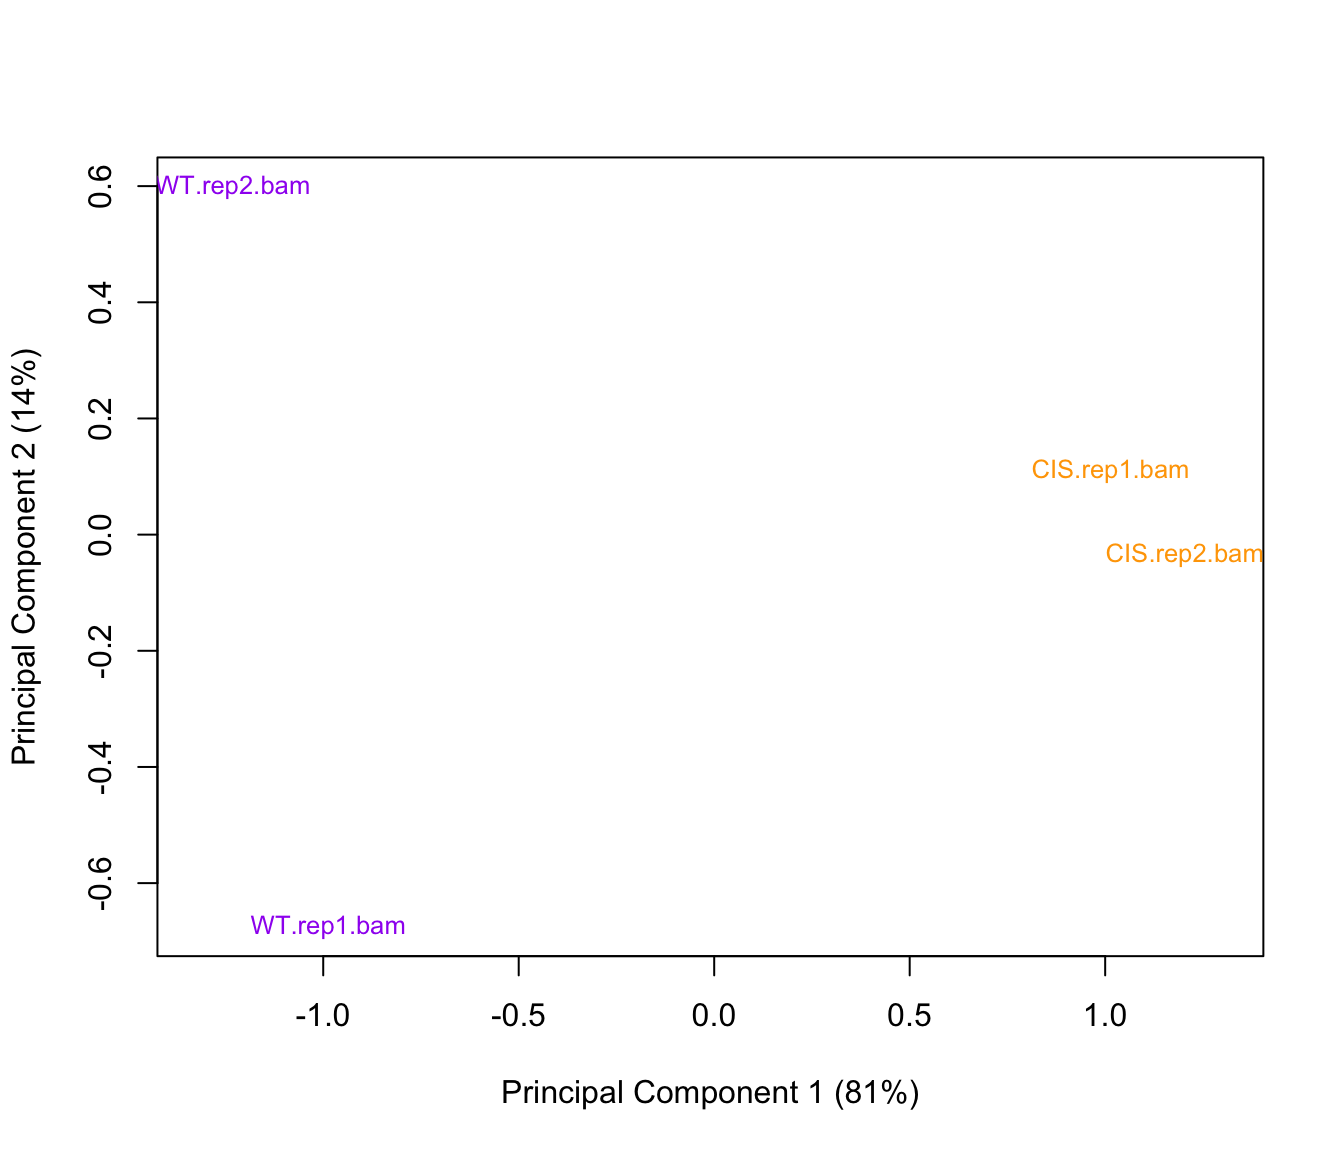
\includegraphics{Bioinfo-figures_files/figure-latex/unnamed-chunk-4-1.pdf}
\#\# Venn diagram

If differential expression analysis is performed on more than 1 comparison, a Venn diagram can be used to quickly compare the number of differentially expressed genes that are either unique to one comparison or DE in other comparisons. This can be easily done using the \textbf{vennDiagram} function in \textbf{limma}.

\hypertarget{mean-difference-plot}{%
\section{Mean-difference plot}\label{mean-difference-plot}}

A mean-difference plot or MD-plot is a plot that can be used to show the fold-change differences against the average expression values of all genes used in the analysis. This can be generated easily using the \emph{plotMD} function within the \textbf{limma} package.

\begin{Shaded}
\begin{Highlighting}[]
\FunctionTok{plotMD}\NormalTok{(fit.contr, }\AttributeTok{column =} \DecValTok{1}\NormalTok{,}\AttributeTok{status =}\NormalTok{ dt,}\AttributeTok{cex=}\FloatTok{0.8}\NormalTok{)}
\end{Highlighting}
\end{Shaded}

\begin{figure}
\centering
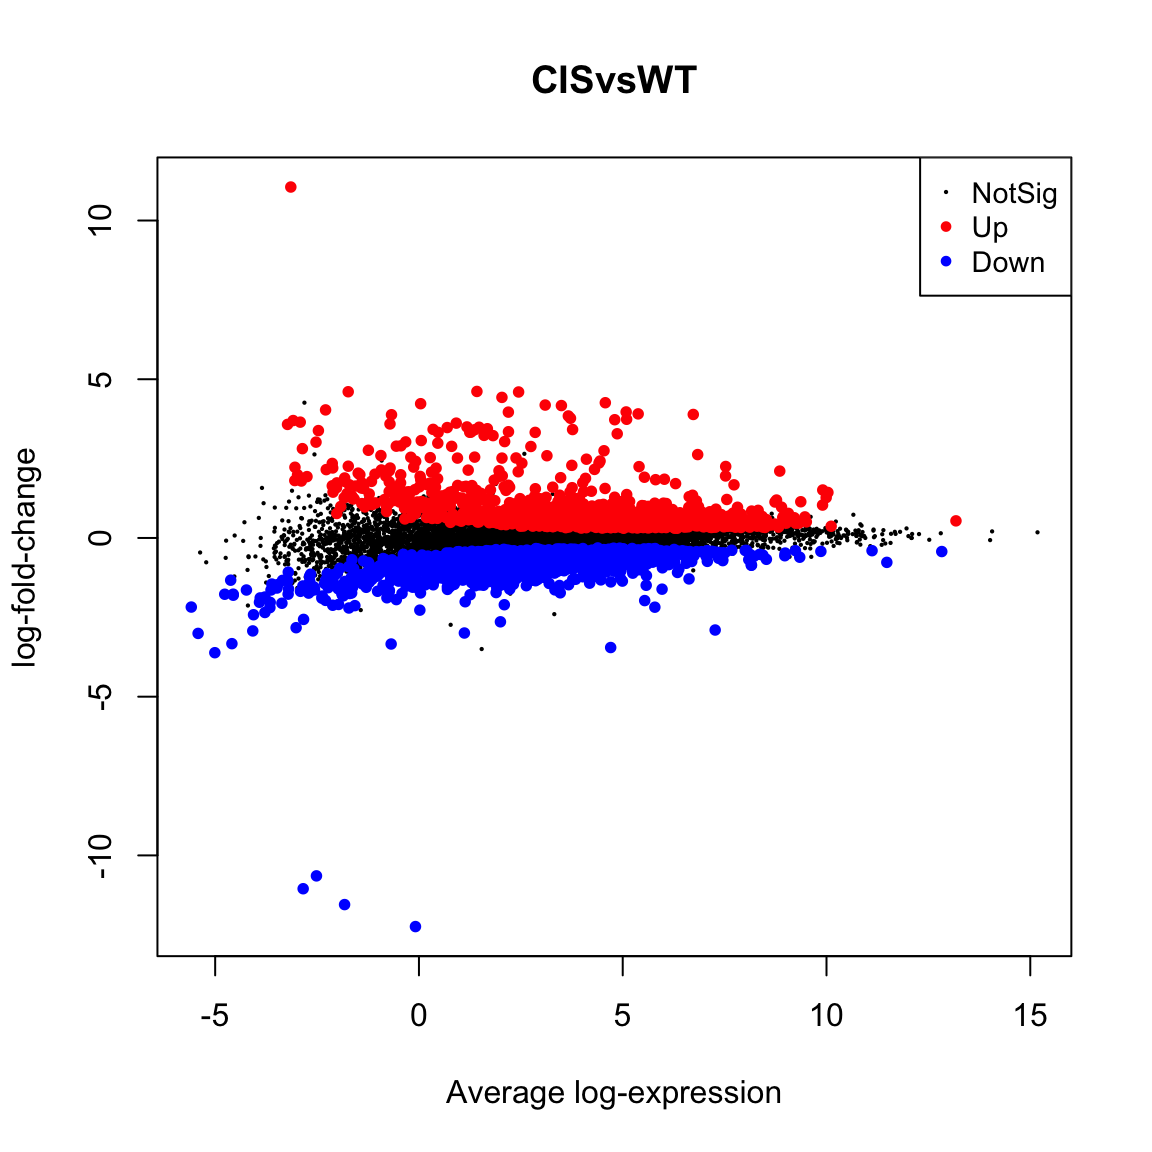
\includegraphics{Bioinfo-figures_files/figure-latex/figmd-1.pdf}
\caption{\label{fig:figmd}Mean-Difference plot. Represents relationship between mean expression and fold-changes}
\end{figure}

\hypertarget{volcano-plots}{%
\section{Volcano plots}\label{volcano-plots}}

A volcano plot shows the relationship between the log fold-change on the x-axis and a measure of statistical significance on the y-axis. The measure of significance can be -log(p-value) or the B-statistics. Here, we will use the \emph{volcanoplot} function within the \textbf{limma} package.In the volcano plot below, differentially expressed genes are highlighted with red for up-regulated and blue for down-regulated genes.

\begin{Shaded}
\begin{Highlighting}[]
\CommentTok{\#highlight de genes}
\NormalTok{col}\OtherTok{\textless{}{-}}\FunctionTok{c}\NormalTok{(}\StringTok{"blue"}\NormalTok{,}\StringTok{"black"}\NormalTok{,}\StringTok{"red"}\NormalTok{)[}\FunctionTok{factor}\NormalTok{(dt[,}\StringTok{"CISvsWT"}\NormalTok{])]}
\FunctionTok{volcanoplot}\NormalTok{(fit.contr,}\AttributeTok{col=}\NormalTok{col)}
\end{Highlighting}
\end{Shaded}

\begin{figure}
\centering
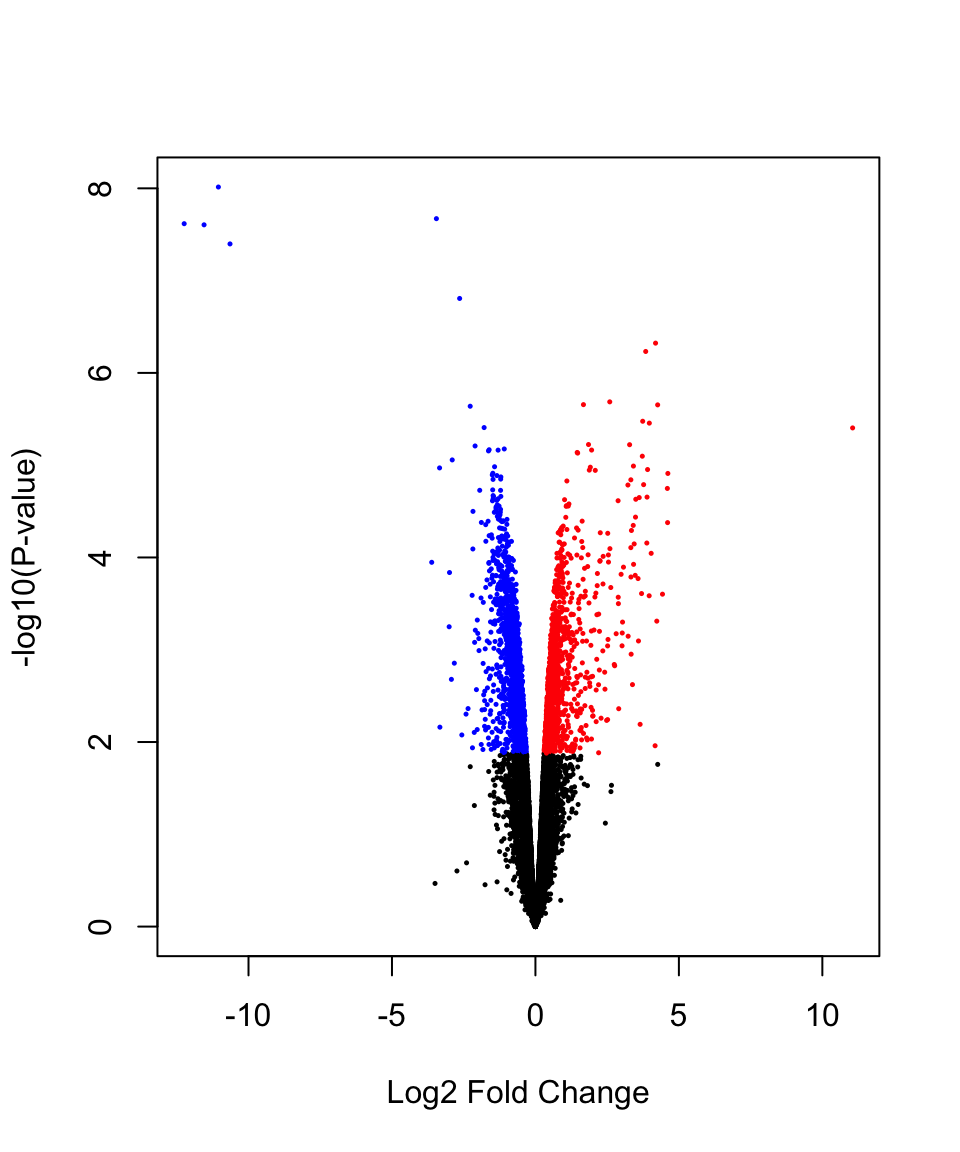
\includegraphics{Bioinfo-figures_files/figure-latex/figvolc-1.pdf}
\caption{\label{fig:figvolc}Volcano plot. Shows the relationship between fold-change and significance of change}
\end{figure}

Alternatively, an interactive mean-difference plot can be generated using \emph{glMDPlot} in \textbf{Glimma} which outputs an interactive html page with results displayed in the left panel and the expression values for the selected gene. A gene within the dataset can be searched through a search bar.

\begin{Shaded}
\begin{Highlighting}[]
\ControlFlowTok{if}\NormalTok{(}\SpecialCharTok{!}\FunctionTok{require}\NormalTok{(Glimma))}
\NormalTok{\{}
\NormalTok{  BiocManager}\SpecialCharTok{::}\FunctionTok{install}\NormalTok{(}\StringTok{"Glimma"}\NormalTok{)}
  \FunctionTok{library}\NormalTok{(Glimma)}
\NormalTok{\}}
\end{Highlighting}
\end{Shaded}

\begin{verbatim}
## Loading required package: Glimma
\end{verbatim}

\begin{Shaded}
\begin{Highlighting}[]
\FunctionTok{glMDPlot}\NormalTok{(fit.contr, }\AttributeTok{coef=}\DecValTok{1}\NormalTok{, }\AttributeTok{status=}\NormalTok{dt, }\AttributeTok{main=}\FunctionTok{colnames}\NormalTok{(fit.contr)[}\DecValTok{1}\NormalTok{],}
         \AttributeTok{side.main=}\StringTok{"ENTREZID"}\NormalTok{, }\AttributeTok{counts=}\NormalTok{y}\SpecialCharTok{$}\NormalTok{E, }\AttributeTok{groups=}\FunctionTok{colnames}\NormalTok{(contr),}
         \AttributeTok{launch =}\NormalTok{ F)}
\end{Highlighting}
\end{Shaded}

\href{glimma-plots/MD-Plot.html}{Click here for interactive version}

Hover over points to see sample-wise expression

\begin{itemize}
\item
  Click on column names to sort by column
\item
  Click rows on tables to highlight gene
\end{itemize}

\hypertarget{heatmaps}{%
\section{Heatmaps}\label{heatmaps}}

Heatmaps are a great way of demonstrating the differences in the expression patterns between different conditions in your dataset. Here we use the \emph{coolmap} function within the \textbf{limma} package which is an extension of the \emph{heatmap.2} function within the \textbf{gplots} package. The heatmap below shows the expression pattern of the top 100 differentially expressed genes between CIS vs WT.

\begin{Shaded}
\begin{Highlighting}[]
\NormalTok{heat.data }\OtherTok{\textless{}{-}}\NormalTok{ y}\SpecialCharTok{$}\NormalTok{E[}\FunctionTok{head}\NormalTok{(}\FunctionTok{rownames}\NormalTok{(de.genes), }\AttributeTok{n =} \DecValTok{100}\NormalTok{), ]}
\FunctionTok{colnames}\NormalTok{(heat.data) }\OtherTok{\textless{}{-}}\NormalTok{ targets}\SpecialCharTok{$}\NormalTok{Sample}
\FunctionTok{rownames}\NormalTok{(heat.data) }\OtherTok{\textless{}{-}} \FunctionTok{head}\NormalTok{(de.genes}\SpecialCharTok{$}\NormalTok{Symbol, }\AttributeTok{n =} \DecValTok{100}\NormalTok{)}
\FunctionTok{coolmap}\NormalTok{(}
\NormalTok{  heat.data,}
  \AttributeTok{margin =} \FunctionTok{c}\NormalTok{(}\DecValTok{5}\NormalTok{, }\DecValTok{4}\NormalTok{),}
  \AttributeTok{cexCol =} \FloatTok{0.8}\NormalTok{,}
  \AttributeTok{lhei =} \FunctionTok{c}\NormalTok{(}\FloatTok{0.8}\NormalTok{, }\DecValTok{4}\NormalTok{),}
  \AttributeTok{cexRow =} \FloatTok{0.6}
\NormalTok{)}
\end{Highlighting}
\end{Shaded}

\begin{figure}
\centering
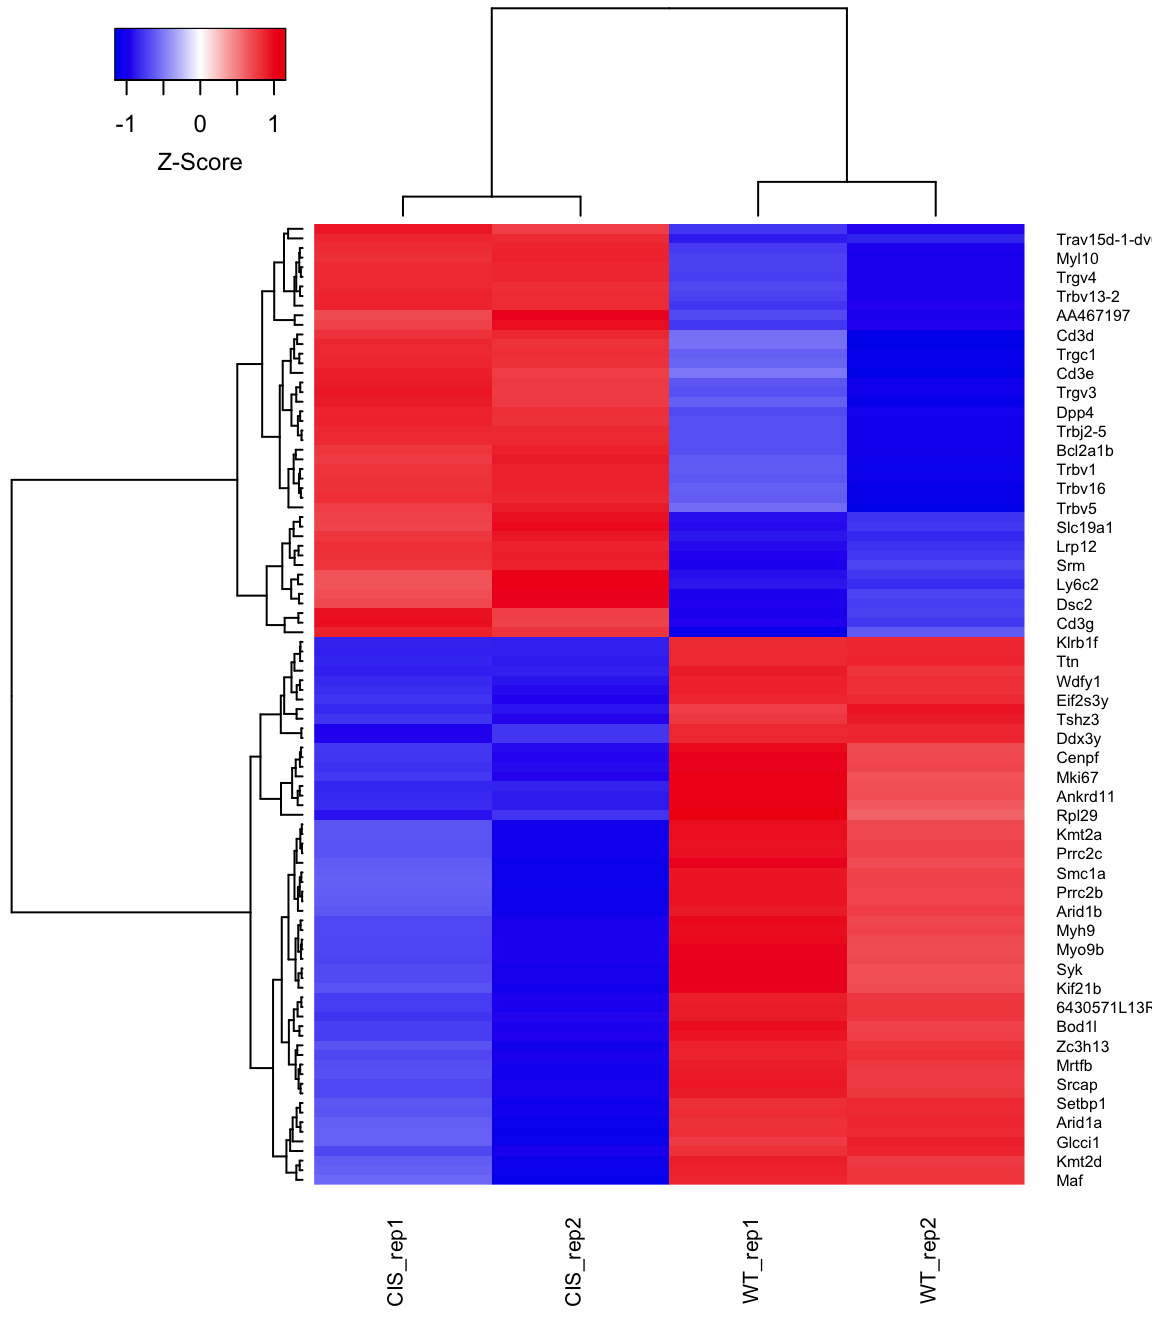
\includegraphics{Bioinfo-figures_files/figure-latex/figheatmap-1.pdf}
\caption{\label{fig:figheatmap}Heatmap plot of differentially expressed genes in CIS vs WT}
\end{figure}

\hypertarget{dendrogram}{%
\section{Dendrogram}\label{dendrogram}}

Similarly we can also use cluster dendrogram to show the relationship between samples.

\begin{Shaded}
\begin{Highlighting}[]
\NormalTok{d}\OtherTok{\textless{}{-}}\FunctionTok{dist}\NormalTok{(}\FunctionTok{t}\NormalTok{(heat.data))}
\NormalTok{hclst}\OtherTok{\textless{}{-}}\FunctionTok{hclust}\NormalTok{(d,}\AttributeTok{method =} \StringTok{"ward.D2"}\NormalTok{)}
\end{Highlighting}
\end{Shaded}

\begin{Shaded}
\begin{Highlighting}[]
\FunctionTok{plot}\NormalTok{(}
\NormalTok{    hclst,}
    \AttributeTok{cex.main =} \DecValTok{1}\NormalTok{,}
    \AttributeTok{cex.lab =} \FloatTok{0.9}\NormalTok{,}
    \AttributeTok{xlab =}\StringTok{""}\NormalTok{,}
    \AttributeTok{cex.axis =} \FloatTok{0.8}\NormalTok{)}
\end{Highlighting}
\end{Shaded}

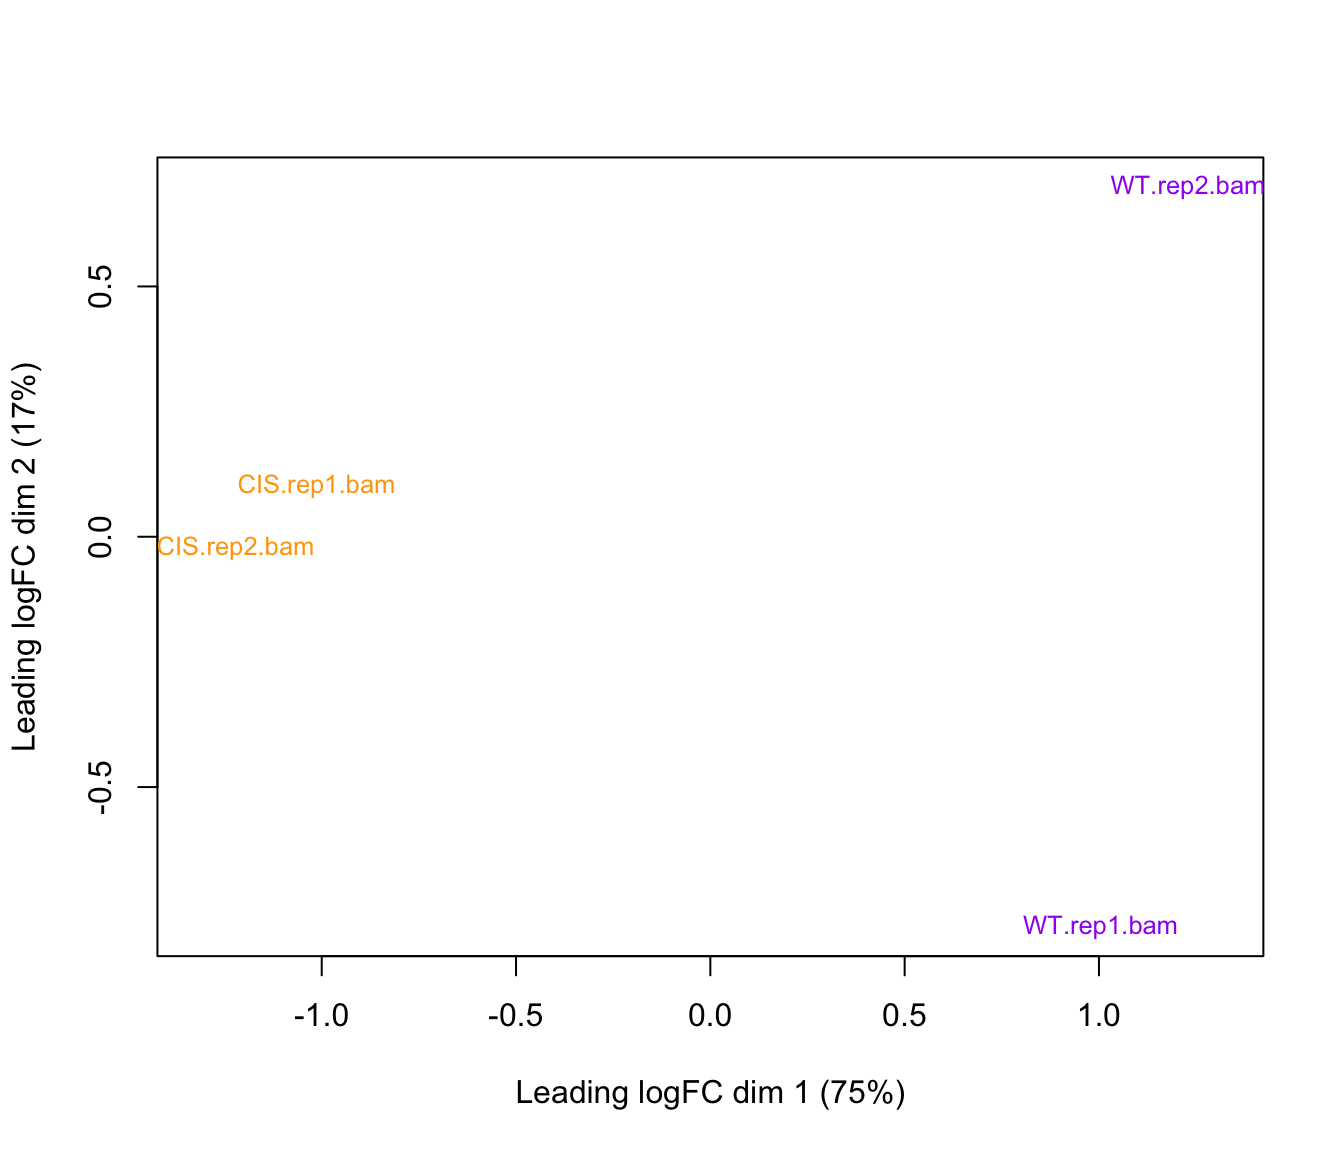
\includegraphics{Bioinfo-figures_files/figure-latex/unnamed-chunk-7-1.pdf}

\hypertarget{pathway-analysis}{%
\section{Pathway Analysis}\label{pathway-analysis}}

From the differential expression analysis there were some 3181 differentially expressed genes. This is quiet a long list of genes to interpret and nearly impossible to go through a gene at a time to gain any meaningful biological understanding. A common downstream analysis step is to understand pathways/gene networks that the genes are implicated in.

\hypertarget{gene-ontology-enrichment}{%
\subsection{Gene Ontology enrichment}\label{gene-ontology-enrichment}}

Gene ontology (\url{http://www.geneontology.org/}) provides a controlled vocabulary for describing biological processes (BP ontology), molecular functions (MF ontology) and cellular components (CC ontology).

The GO ontologies themselves are organism-independent; terms are associated with genes for a specific organism through direct experimentation or through sequence homology with another organism and its GO annotation.

Terms are related to other terms through parent-child relationships in a directed acylic graph.

You can use enrichment analysis as another way of drawing conclusions from your set of differentially expressed genes.

\begin{Shaded}
\begin{Highlighting}[]
\NormalTok{enrich.pvalue}\OtherTok{\textless{}{-}}\FloatTok{0.00001}
\end{Highlighting}
\end{Shaded}

Here, we use the \emph{goana} function within the \textbf{limma} package to test for enrichment of differentially expressed genes between the CIS vs WT. Note that the \emph{p-values} returned by \emph{goana} are \textbf{unadjusted for multiple testing}. It is therfore, advisable that if the results are to be published, only terms with very small p-values should be included. For instance, in the example below, only terms with a p-value \textless{} \ensuremath{10^{-5}} are retained.

We use the output from the differential expression analysis and test for overrepresentation for the Up and Down regulated genes separately.

\begin{Shaded}
\begin{Highlighting}[]
\ControlFlowTok{if}\NormalTok{(}\SpecialCharTok{!}\FunctionTok{requireNamespace}\NormalTok{(}\StringTok{"GO.db"}\NormalTok{))}
\NormalTok{  BiocManager}\SpecialCharTok{::}\FunctionTok{install}\NormalTok{(}\StringTok{"GO.db"}\NormalTok{)}
\FunctionTok{library}\NormalTok{(GO.db)}
\NormalTok{go.rst}\OtherTok{\textless{}{-}}\FunctionTok{goana}\NormalTok{(fit.contr,}\AttributeTok{species=}\StringTok{"Mm"}\NormalTok{)}
\CommentTok{\#exclude terms not meeting our cut{-}off}
\NormalTok{go.rst}\OtherTok{\textless{}{-}}\NormalTok{go.rst[}\FunctionTok{rowSums}\NormalTok{(go.rst[,}\FunctionTok{c}\NormalTok{(}\StringTok{"P.Up"}\NormalTok{,}\StringTok{"P.Down"}\NormalTok{)]}\SpecialCharTok{\textless{}}\NormalTok{enrich.pvalue)}\SpecialCharTok{==}\DecValTok{1}\NormalTok{,]}
\end{Highlighting}
\end{Shaded}

A simple way to visualize the enrichment results is through a bar plot as shown below which shows the top 10 enriched terms in each direction.

\begin{Shaded}
\begin{Highlighting}[]
\NormalTok{top.up }\OtherTok{\textless{}{-}} \FunctionTok{head}\NormalTok{(go.rst[}\FunctionTok{order}\NormalTok{(go.rst}\SpecialCharTok{$}\NormalTok{P.Up, }\AttributeTok{decreasing =}\NormalTok{ F),], }\AttributeTok{n =} \DecValTok{10}\NormalTok{)}
\NormalTok{top.down }\OtherTok{\textless{}{-}}
  \FunctionTok{head}\NormalTok{(go.rst[}\FunctionTok{order}\NormalTok{(go.rst}\SpecialCharTok{$}\NormalTok{P.Down, }\AttributeTok{decreasing =}\NormalTok{ F),], }\AttributeTok{n =} \DecValTok{10}\NormalTok{)}
\NormalTok{bar.data }\OtherTok{\textless{}{-}}
  \FunctionTok{rbind}\NormalTok{(}
    \FunctionTok{data.frame}\NormalTok{(}
      \AttributeTok{Term =}\NormalTok{ top.up}\SpecialCharTok{$}\NormalTok{Term,}
      \AttributeTok{P.value =}\NormalTok{ top.up}\SpecialCharTok{$}\NormalTok{P.Up,}
      \AttributeTok{Dir =} \StringTok{"up"}
\NormalTok{    ),}
    \FunctionTok{data.frame}\NormalTok{(}
      \AttributeTok{Term =}\NormalTok{ top.down}\SpecialCharTok{$}\NormalTok{Term,}
      \AttributeTok{P.value =}\NormalTok{ top.down}\SpecialCharTok{$}\NormalTok{P.Down,}
      \AttributeTok{Dir =} \StringTok{"down"}
\NormalTok{    )}
\NormalTok{  )}
\NormalTok{bar.data }\OtherTok{\textless{}{-}}\NormalTok{ bar.data[}\FunctionTok{order}\NormalTok{(bar.data}\SpecialCharTok{$}\NormalTok{P.value, }\AttributeTok{decreasing =}\NormalTok{ F),]}
\FunctionTok{par}\NormalTok{(}\AttributeTok{mai =} \FunctionTok{c}\NormalTok{(}\FloatTok{0.8}\NormalTok{, }\DecValTok{2}\NormalTok{, }\FloatTok{0.5}\NormalTok{, }\FloatTok{0.5}\NormalTok{))}
\NormalTok{bb }\OtherTok{\textless{}{-}} \FunctionTok{barplot}\NormalTok{(}
  \SpecialCharTok{{-}}\FunctionTok{log10}\NormalTok{(bar.data}\SpecialCharTok{$}\NormalTok{P.value),}
  \AttributeTok{horiz =}\NormalTok{ T,}
  \AttributeTok{xlab =} \StringTok{" {-}log10(p{-}value)"}\NormalTok{,}
  \AttributeTok{cex.names =} \FloatTok{0.5}\NormalTok{,}
  \AttributeTok{col =} \FunctionTok{c}\NormalTok{(}\StringTok{"red"}\NormalTok{, }\StringTok{"blue"}\NormalTok{)[}\FunctionTok{factor}\NormalTok{(bar.data}\SpecialCharTok{$}\NormalTok{Dir)]}
\NormalTok{)}
\FunctionTok{axis}\NormalTok{(}
  \DecValTok{2}\NormalTok{,}
  \AttributeTok{line =} \SpecialCharTok{{-}}\FloatTok{0.8}\NormalTok{,}
  \AttributeTok{at =}\NormalTok{ bb,}
  \AttributeTok{labels =}\NormalTok{ bar.data}\SpecialCharTok{$}\NormalTok{Term,}
  \AttributeTok{tick =}\NormalTok{ F,}
  \AttributeTok{las =} \DecValTok{2}\NormalTok{,}
  \AttributeTok{cex.axis =} \FloatTok{0.5}
\NormalTok{)}
\FunctionTok{legend}\NormalTok{(}\StringTok{"topright"}\NormalTok{,}\AttributeTok{legend =} \FunctionTok{c}\NormalTok{(}\StringTok{"Up"}\NormalTok{,}\StringTok{"Down"}\NormalTok{),}\AttributeTok{pch =} \DecValTok{22}\NormalTok{,}\AttributeTok{pt.bg =} \FunctionTok{c}\NormalTok{(}\StringTok{"red"}\NormalTok{,}\StringTok{"blue"}\NormalTok{))}
\end{Highlighting}
\end{Shaded}

\begin{figure}
\centering
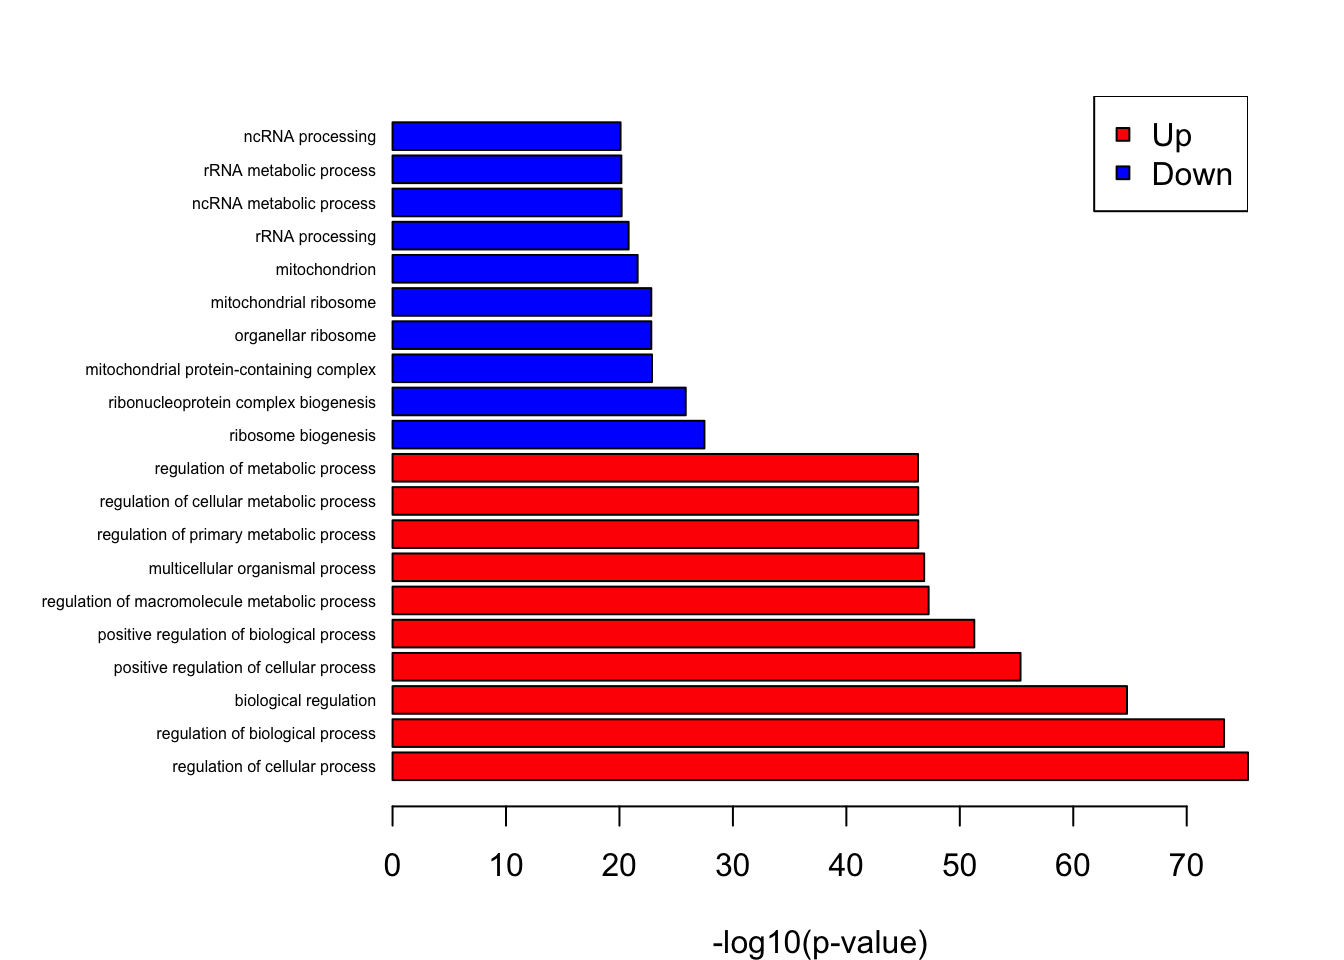
\includegraphics{Bioinfo-figures_files/figure-latex/enrichplot-1.pdf}
\caption{\label{fig:enrichplot}Enrichment plot. Top enrichments in either direction}
\end{figure}

\textbf{Add gene information (optional)}

Sometimes you may want to know what genes are enriched in each of the terms, this section allows you to add gene details.

First, we extract the genes that are associated with the catalytic activity GO terms. This results in a list mapping the GO term and the associated genes.

\begin{Shaded}
\begin{Highlighting}[]
\ControlFlowTok{if}\NormalTok{(}\SpecialCharTok{!}\FunctionTok{require}\NormalTok{(GO.db))}
\NormalTok{  BiocManager}\SpecialCharTok{::}\FunctionTok{install}\NormalTok{(}\StringTok{"GO.db"}\NormalTok{)}
\ControlFlowTok{if}\NormalTok{(}\SpecialCharTok{!}\FunctionTok{require}\NormalTok{(org.Mm.eg.db))}
\NormalTok{  BiocManager}\SpecialCharTok{::}\FunctionTok{install}\NormalTok{(}\StringTok{"org.Mm.eg.db"}\NormalTok{)}
\end{Highlighting}
\end{Shaded}

\begin{verbatim}
## Loading required package: org.Mm.eg.db
\end{verbatim}

\begin{Shaded}
\begin{Highlighting}[]
\NormalTok{go.EntrezID }\OtherTok{\textless{}{-}} \FunctionTok{as.list}\NormalTok{(org.Mm.egGO2ALLEGS)}
\NormalTok{go.rst }\OtherTok{\textless{}{-}}\NormalTok{ tibble}\SpecialCharTok{::}\FunctionTok{rownames\_to\_column}\NormalTok{(go.rst, }\AttributeTok{var =} \StringTok{"GO.ID"}\NormalTok{)}
\end{Highlighting}
\end{Shaded}

\begin{Shaded}
\begin{Highlighting}[]
\CommentTok{\#Add gene details}
\NormalTok{go.rst}\SpecialCharTok{$}\NormalTok{Genes.Up }\OtherTok{\textless{}{-}} \FunctionTok{unlist}\NormalTok{(}\FunctionTok{lapply}\NormalTok{(go.rst}\SpecialCharTok{$}\NormalTok{GO.ID, }\ControlFlowTok{function}\NormalTok{(x) \{}
\NormalTok{  xx }\OtherTok{\textless{}{-}}\NormalTok{ go.EntrezID[[x]]}
  \ControlFlowTok{if}\NormalTok{ (}\FunctionTok{is.null}\NormalTok{(xx) }\SpecialCharTok{|}
      \FunctionTok{with}\NormalTok{(go.rst[go.rst}\SpecialCharTok{$}\NormalTok{GO.ID }\SpecialCharTok{==}\NormalTok{ x,], Up }\SpecialCharTok{==} \DecValTok{0} \SpecialCharTok{|}
\NormalTok{           P.Up }\SpecialCharTok{\textgreater{}}\NormalTok{ enrich.pvalue))}
    \FunctionTok{return}\NormalTok{(}\StringTok{"{-}"}\NormalTok{)}
\NormalTok{  x }\OtherTok{\textless{}{-}} \FunctionTok{intersect}\NormalTok{(}\FunctionTok{with}\NormalTok{(de.genes,EntrezID[logFC}\SpecialCharTok{\textgreater{}}\DecValTok{0}\NormalTok{]),xx)}
\NormalTok{  x }\OtherTok{\textless{}{-}}
    \FunctionTok{paste0}\NormalTok{(}\FunctionTok{with}\NormalTok{(fit.contr}\SpecialCharTok{$}\NormalTok{genes, Symbol[EntrezID }\SpecialCharTok{\%in\%}\NormalTok{ xx]), }\AttributeTok{collapse =} \StringTok{"|"}\NormalTok{)}
  \FunctionTok{return}\NormalTok{(x)}
\NormalTok{\}))}
\NormalTok{go.rst}\SpecialCharTok{$}\NormalTok{Genes.Down }\OtherTok{\textless{}{-}} \FunctionTok{unlist}\NormalTok{(}\FunctionTok{lapply}\NormalTok{(go.rst}\SpecialCharTok{$}\NormalTok{GO.ID, }\ControlFlowTok{function}\NormalTok{(x) \{}
\NormalTok{  xx }\OtherTok{\textless{}{-}}\NormalTok{ go.EntrezID[[x]]}
  \ControlFlowTok{if}\NormalTok{ (}\FunctionTok{is.null}\NormalTok{(xx) }\SpecialCharTok{|}
      \FunctionTok{with}\NormalTok{(go.rst[go.rst}\SpecialCharTok{$}\NormalTok{GO.ID }\SpecialCharTok{==}\NormalTok{ x,], Down }\SpecialCharTok{==} \DecValTok{0} \SpecialCharTok{|}
\NormalTok{           P.Down }\SpecialCharTok{\textgreater{}}\NormalTok{ enrich.pvalue))}
    \FunctionTok{return}\NormalTok{(}\StringTok{"{-}"}\NormalTok{)}
\NormalTok{  x }\OtherTok{\textless{}{-}} \FunctionTok{intersect}\NormalTok{(}\FunctionTok{with}\NormalTok{(de.genes,EntrezID[logFC}\SpecialCharTok{\textless{}}\DecValTok{0}\NormalTok{]),xx)}
\NormalTok{  x }\OtherTok{\textless{}{-}}
    \FunctionTok{paste0}\NormalTok{(}\FunctionTok{with}\NormalTok{(fit.contr}\SpecialCharTok{$}\NormalTok{genes, Symbol[EntrezID }\SpecialCharTok{\%in\%}\NormalTok{ xx]), }\AttributeTok{collapse =} \StringTok{"|"}\NormalTok{)}
  \FunctionTok{return}\NormalTok{(x)}
\NormalTok{\}))}
\end{Highlighting}
\end{Shaded}

\hypertarget{kegg-pathway-enrichment}{%
\subsection{KEGG pathway enrichment}\label{kegg-pathway-enrichment}}

Pathway enrichment can also be performed against the Kyoto Encyclopedia of Genes and Genomes (KEGG) (\url{https://www.genome.jp/kegg/}) database. The KEGG database contains curated molecular pathways and disease signatures. To perform this analysis we use the \emph{kegga} function within the \textbf{limma} which is similar to the \emph{goana} function we used above.

\begin{Shaded}
\begin{Highlighting}[]
\NormalTok{kegg.rst}\OtherTok{\textless{}{-}}\FunctionTok{kegga}\NormalTok{(fit.contr,}\AttributeTok{species=}\StringTok{"Mm"}\NormalTok{)}
\FunctionTok{topKEGG}\NormalTok{(kegg.rst)}
\end{Highlighting}
\end{Shaded}

\begin{verbatim}
##                                               Pathway    N  Up Down
## path:mmu03008       Ribosome biogenesis in eukaryotes   75  37    4
## path:mmu01100                      Metabolic pathways 1038 206   75
## path:mmu04810        Regulation of actin cytoskeleton  143   6   45
## path:mmu05206                     MicroRNAs in cancer  121   6   40
## path:mmu04919       Thyroid hormone signaling pathway   93   3   32
## path:mmu03010                                Ribosome  137  39    1
## path:mmu01240               Biosynthesis of cofactors  111  32    2
## path:mmu04330                 Notch signaling pathway   43   2   18
## path:mmu00310                      Lysine degradation   52   1   20
## path:mmu03020                          RNA polymerase   32  14    1
## path:mmu00190               Oxidative phosphorylation  118  32    0
## path:mmu04062             Chemokine signaling pathway  119   5   34
## path:mmu04611                     Platelet activation   77   0   25
## path:mmu05200                      Pathways in cancer  323  26   71
## path:mmu05205                 Proteoglycans in cancer  126   8   34
## path:mmu04658        Th1 and Th2 cell differentiation   69   6   22
## path:mmu05224                           Breast cancer   81   8   24
## path:mmu05202 Transcriptional misregulation in cancer  121  16   32
## path:mmu03050                              Proteasome   44  15    0
## path:mmu01232                   Nucleotide metabolism   65  19    0
##                       P.Up       P.Down
## path:mmu03008 1.182585e-14 9.951210e-01
## path:mmu01100 5.674601e-12 1.000000e+00
## path:mmu04810 9.998630e-01 4.679254e-08
## path:mmu05206 9.987434e-01 5.746746e-08
## path:mmu04919 9.996663e-01 4.319019e-07
## path:mmu03010 6.123733e-07 1.000000e+00
## path:mmu01240 4.561006e-06 9.999989e-01
## path:mmu04330 9.789811e-01 6.418221e-06
## path:mmu00310 9.991527e-01 9.325271e-06
## path:mmu03020 1.341355e-05 9.916924e-01
## path:mmu00190 1.832128e-05 1.000000e+00
## path:mmu04062 9.995796e-01 2.081620e-05
## path:mmu04611 1.000000e+00 2.435669e-05
## path:mmu05200 9.971966e-01 4.089375e-05
## path:mmu05205 9.933378e-01 7.494761e-05
## path:mmu04658 8.861202e-01 1.000116e-04
## path:mmu05224 8.230146e-01 1.784375e-04
## path:mmu05202 4.708773e-01 1.811724e-04
## path:mmu03050 2.086057e-04 1.000000e+00
## path:mmu01232 3.146027e-04 1.000000e+00
\end{verbatim}

\hypertarget{gene-set-enrichment-analysis}{%
\subsection{Gene Set Enrichment Analysis}\label{gene-set-enrichment-analysis}}

GO and KEGG enrichment analysis uses the list of differentially expressed genes to test for over-representation of these genes. As such the results typically depend on the cut-offs used to get the differentially expressed genes.

Gene Set Enrichment Analysis is performed using \emph{roast}, a gene set enrichment function within the \textbf{limma} package. Unlike above where we focused on a subset of genes(differentially genes), here all the genes in the set are used to test for gene expression signatures or pathways. A test is performed against the GO terms for demonstrative purposes, alternatively, if you wish to test against a specific gene set, this can quickly be done by importing that list.

We then use \emph{roast} to test for enrichment between CIS and WT. We use the design matrix `design', the expression values `y' and the contrast matrix `contr' from the imported results to perform the gene set test and the GO term and gene map we created above.

\begin{Shaded}
\begin{Highlighting}[]
\NormalTok{go.all}\OtherTok{\textless{}{-}}\NormalTok{go.EntrezID[go.rst}\SpecialCharTok{$}\NormalTok{GO.ID]}
\FunctionTok{names}\NormalTok{(go.all)}\OtherTok{\textless{}{-}}\NormalTok{go.rst}\SpecialCharTok{$}\NormalTok{Term}
\NormalTok{roast.GSEA}\OtherTok{\textless{}{-}}\FunctionTok{roast}\NormalTok{(y,}\AttributeTok{index =}\NormalTok{ go.all,}\AttributeTok{design =}\NormalTok{ design,}\AttributeTok{contrast =}\NormalTok{ contr)}
\FunctionTok{head}\NormalTok{(roast.GSEA)}
\end{Highlighting}
\end{Shaded}

\begin{verbatim}
##                                      NGenes   PropDown    PropUp Direction
## 90S preribosome                          28 0.07142857 0.7142857        Up
## RNA processing                          809 0.26205192 0.4066749        Up
## preribosome                              79 0.06329114 0.6708861        Up
## meiotic chromosome segregation           63 0.55555556 0.0952381      Down
## mitotic sister chromatid segregation    150 0.52000000 0.1666667      Down
## regulation of chromosome separation      69 0.47826087 0.1884058      Down
##                                      PValue       FDR PValue.Mixed  FDR.Mixed
## 90S preribosome                      0.0005 0.1000000       0.0060 0.06227709
## RNA processing                       0.0005 0.1000000       0.0555 0.06227709
## preribosome                          0.0020 0.1253906       0.0130 0.06227709
## meiotic chromosome segregation       0.0035 0.1253906       0.0210 0.06227709
## mitotic sister chromatid segregation 0.0035 0.1253906       0.0135 0.06227709
## regulation of chromosome separation  0.0035 0.1253906       0.0160 0.06227709
\end{verbatim}

\begin{Shaded}
\begin{Highlighting}[]
\NormalTok{term.test}\OtherTok{\textless{}{-}}\FunctionTok{rownames}\NormalTok{(roast.GSEA)[}\DecValTok{1}\NormalTok{]}
\end{Highlighting}
\end{Shaded}

Next, we can visualize the gene set enrichment results using a barcode plot. The barcode plot is used to plot the positions of genes within a set in ranked list of statistics. The statistics are ranked from left to right ie. from smallest to largest.

To do so, the gene identifies for the term should first be mapped to the index position of each gene in the expression matrix;

\begin{Shaded}
\begin{Highlighting}[]
\NormalTok{index }\OtherTok{\textless{}{-}} \FunctionTok{rownames}\NormalTok{(fit.contr) }\SpecialCharTok{\%in\%}\NormalTok{ go.all[[}\FunctionTok{rownames}\NormalTok{(roast.GSEA)[}\DecValTok{1}\NormalTok{]]]}
\FunctionTok{barcodeplot}\NormalTok{(}
\NormalTok{  fit.contr}\SpecialCharTok{$}\NormalTok{coefficients[, }\StringTok{"CISvsWT"}\NormalTok{],}
  \AttributeTok{index =}\NormalTok{ index,}
  \AttributeTok{labels =} \FunctionTok{c}\NormalTok{(}\StringTok{"CS"}\NormalTok{, }\StringTok{"WT"}\NormalTok{),}
  \AttributeTok{main =} \FunctionTok{rownames}\NormalTok{(roast.GSEA)[}\DecValTok{1}\NormalTok{]}
\NormalTok{)}
\end{Highlighting}
\end{Shaded}

\begin{figure}
\centering
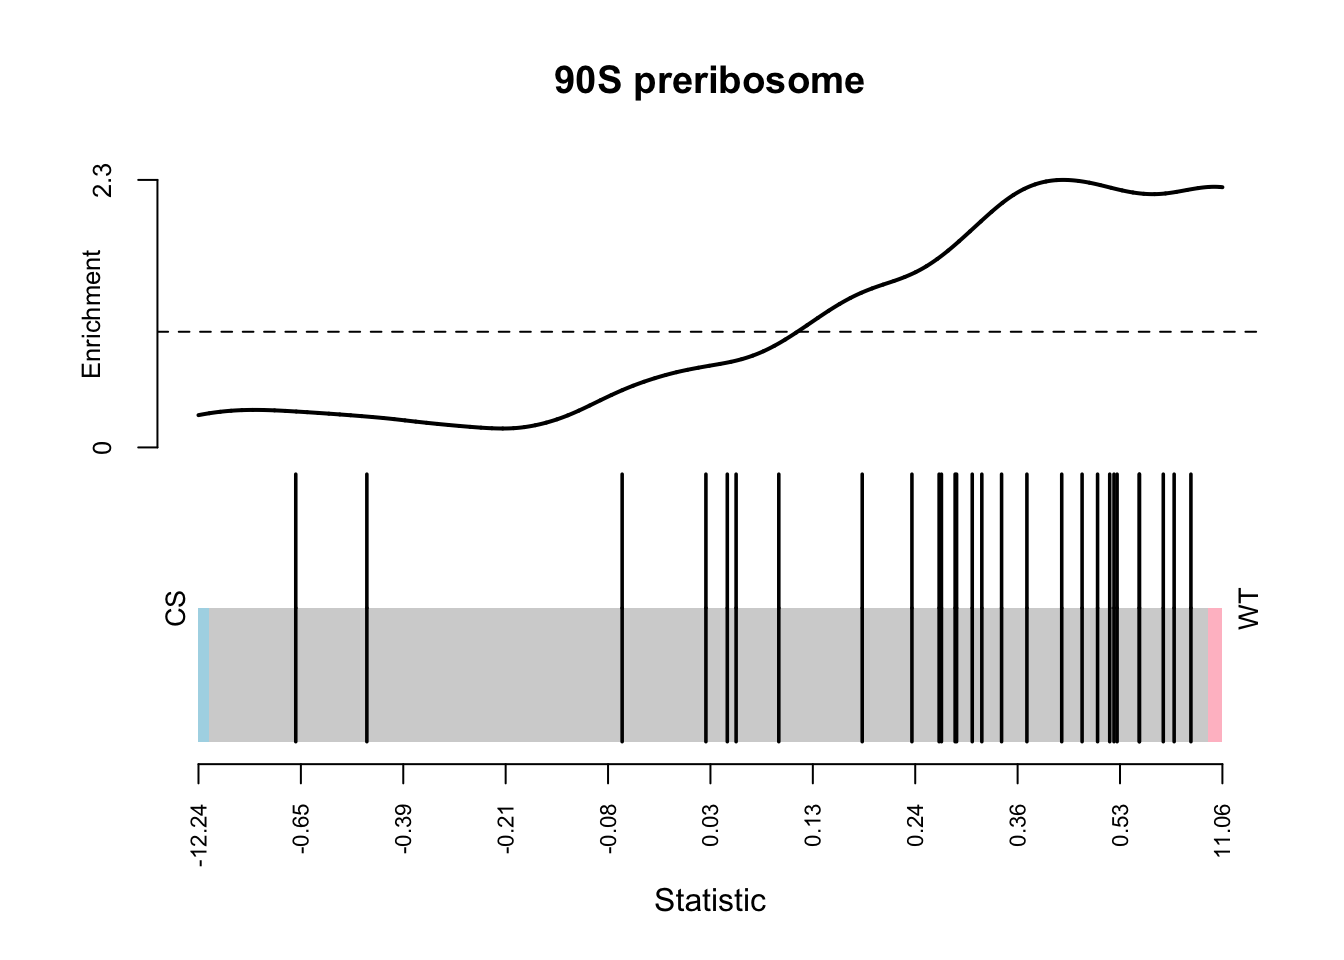
\includegraphics{Bioinfo-figures_files/figure-latex/unnamed-chunk-15-1.pdf}
\caption{\label{fig:unnamed-chunk-15}Barcode plot showing the enrichment of 90S preribosome in CS vs WT}
\end{figure}

\vspace{-100pt}

\vspace{-100pt}

\hypertarget{scrna-seq-data-1}{%
\chapter{scRNA-seq data}\label{scrna-seq-data-1}}

\hypertarget{background-1}{%
\section{Background}\label{background-1}}

As discussed previously, processed counts from the \href{https://chisangad.github.io/scRNAseqtut/index.html}{scRNA-seq workshop} are used here to demonstrate the different types of figures that can be generated for publications.

\hypertarget{tsne-plots}{%
\section{tSNE plots}\label{tsne-plots}}

t-distributed stochastic neighbor embedding (t-SNE) is a statistical method for visualizing high-dimensional data by giving each data point a location in a two or three-dimensional map. It is a dimensionality reduction technique which is a way to graphically simplify very large datasets.

\begin{Shaded}
\begin{Highlighting}[]
\FunctionTok{library}\NormalTok{(Seurat)}
\end{Highlighting}
\end{Shaded}

\begin{verbatim}
## Attaching SeuratObject
\end{verbatim}

\begin{verbatim}
## Attaching sp
\end{verbatim}

\begin{Shaded}
\begin{Highlighting}[]
\FunctionTok{library}\NormalTok{(ggplot2)}
\FunctionTok{load}\NormalTok{(}\StringTok{"Counts\_scRNA{-}norm.RData"}\NormalTok{)}
\end{Highlighting}
\end{Shaded}

\begin{Shaded}
\begin{Highlighting}[]
\FunctionTok{DimPlot}\NormalTok{(}
\NormalTok{  counts\_st,}
  \AttributeTok{reduction =} \StringTok{"tsne"}\NormalTok{,}
  \AttributeTok{label =}\NormalTok{ T,}
  \AttributeTok{size =} \FloatTok{0.5}\NormalTok{,}
  \AttributeTok{repel =}\NormalTok{ T,}
  \AttributeTok{cols =} \FunctionTok{DiscretePalette}\NormalTok{(}\FunctionTok{length}\NormalTok{(}\FunctionTok{levels}\NormalTok{(}\FunctionTok{Idents}\NormalTok{(}
\NormalTok{    counts\_st}
\NormalTok{  ))))}
\NormalTok{)}
\end{Highlighting}
\end{Shaded}

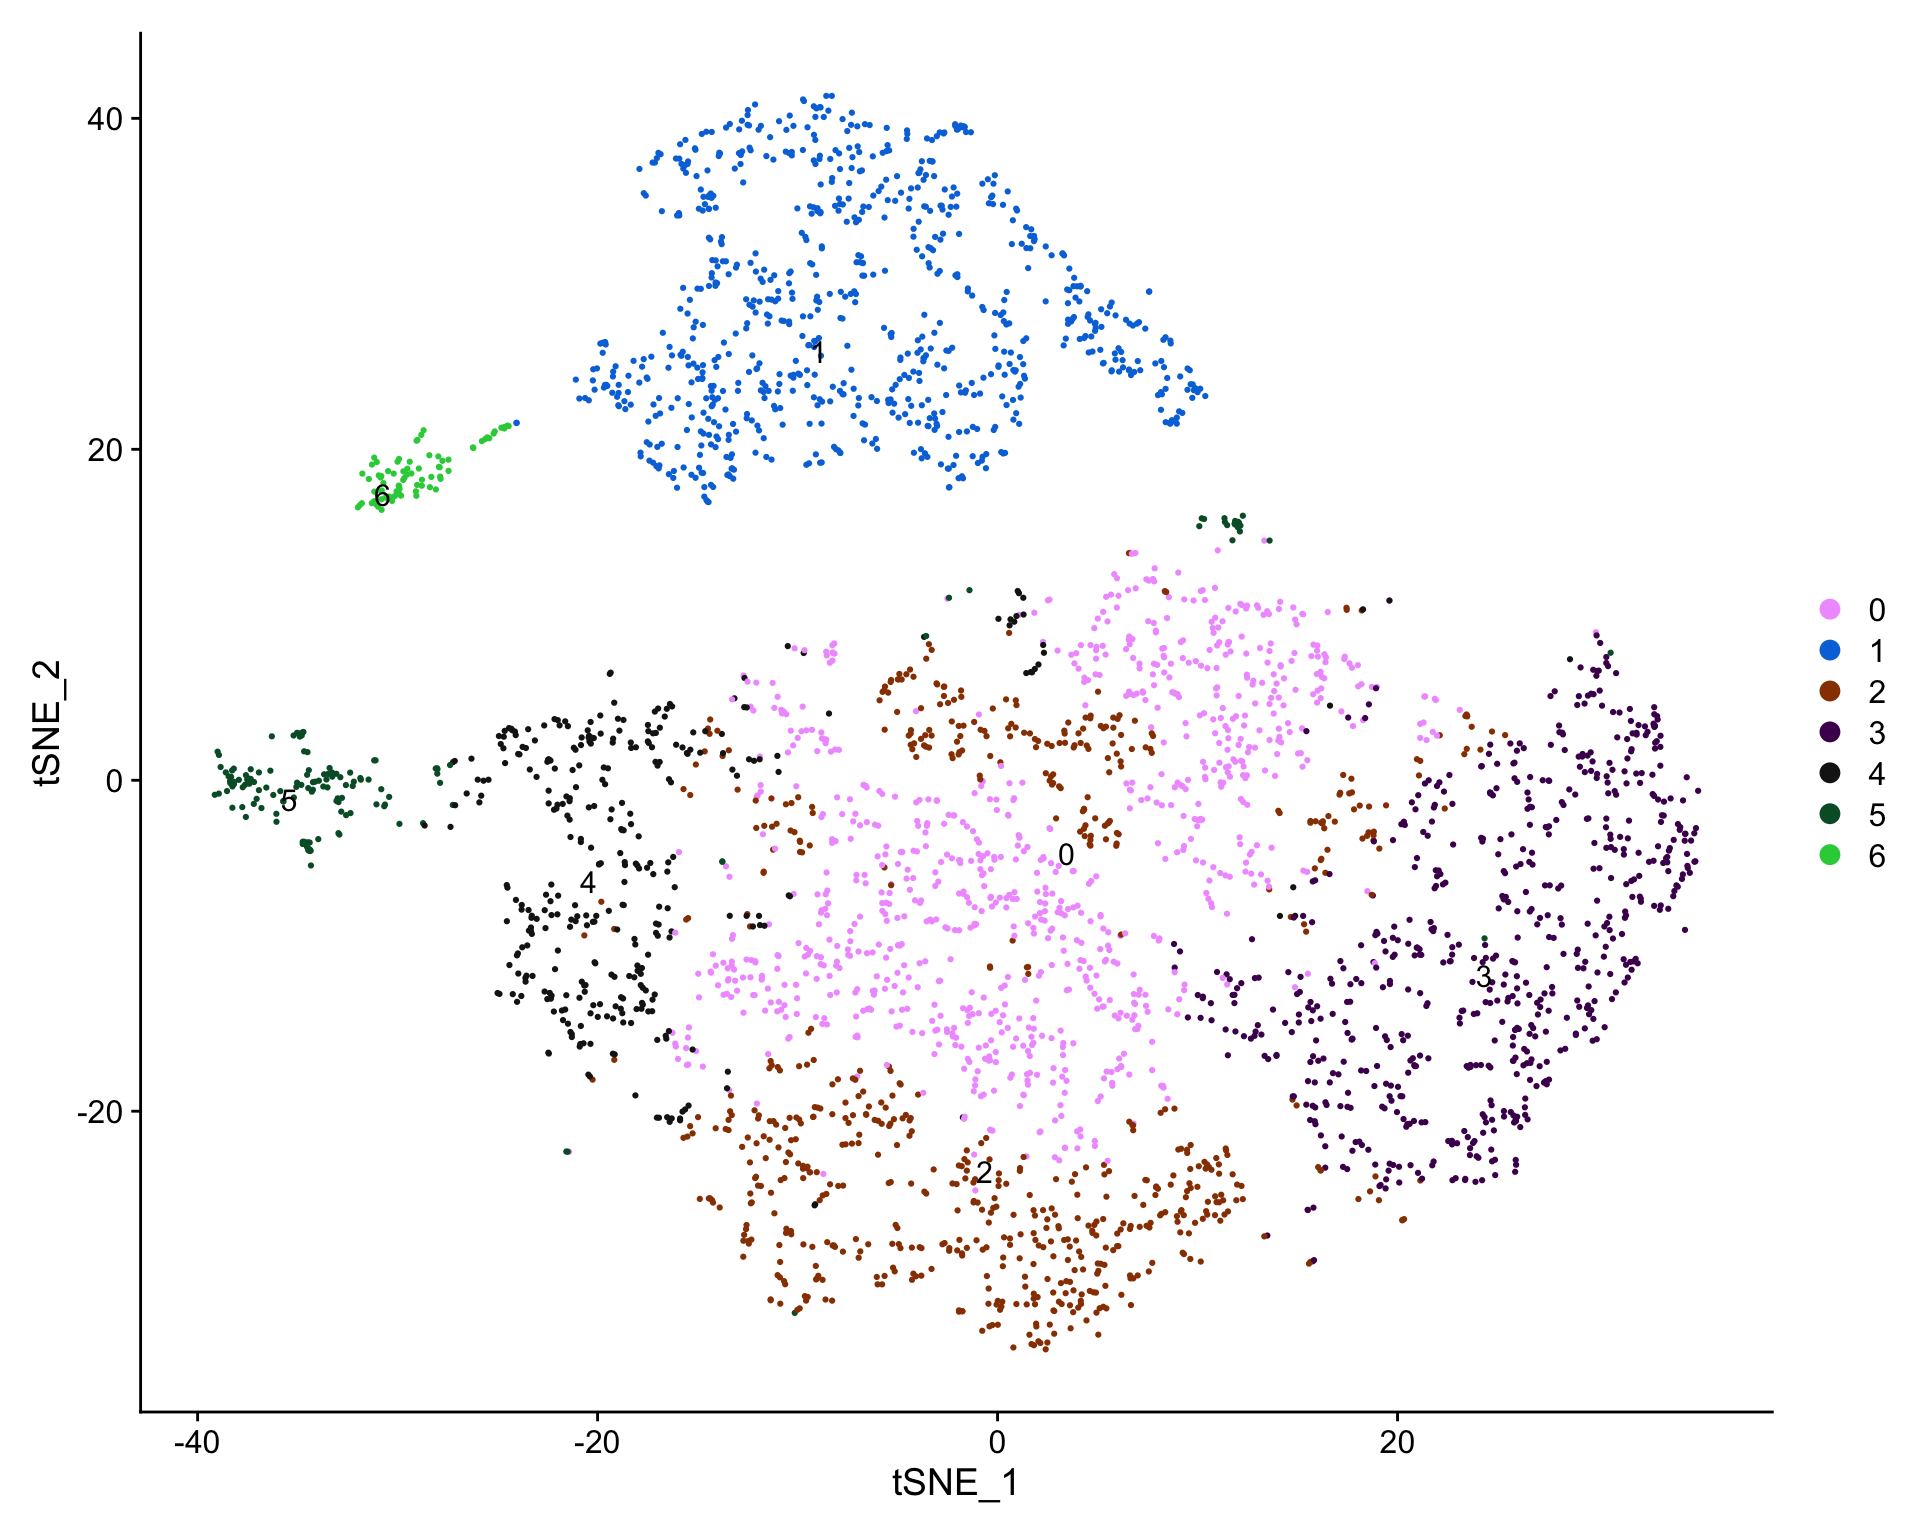
\includegraphics{Bioinfo-figures_files/figure-latex/unnamed-chunk-17-1.pdf}

\begin{Shaded}
\begin{Highlighting}[]
\FunctionTok{DimPlot}\NormalTok{(}
\NormalTok{  counts\_st,}
  \AttributeTok{reduction =} \StringTok{"tsne"}\NormalTok{,}
  \AttributeTok{label =}\NormalTok{ T,}
  \AttributeTok{group.by =} \StringTok{"Sample"}\NormalTok{,}
  \AttributeTok{size =} \FloatTok{0.5}\NormalTok{,}
  \AttributeTok{repel =}\NormalTok{ T}
\NormalTok{)}
\end{Highlighting}
\end{Shaded}

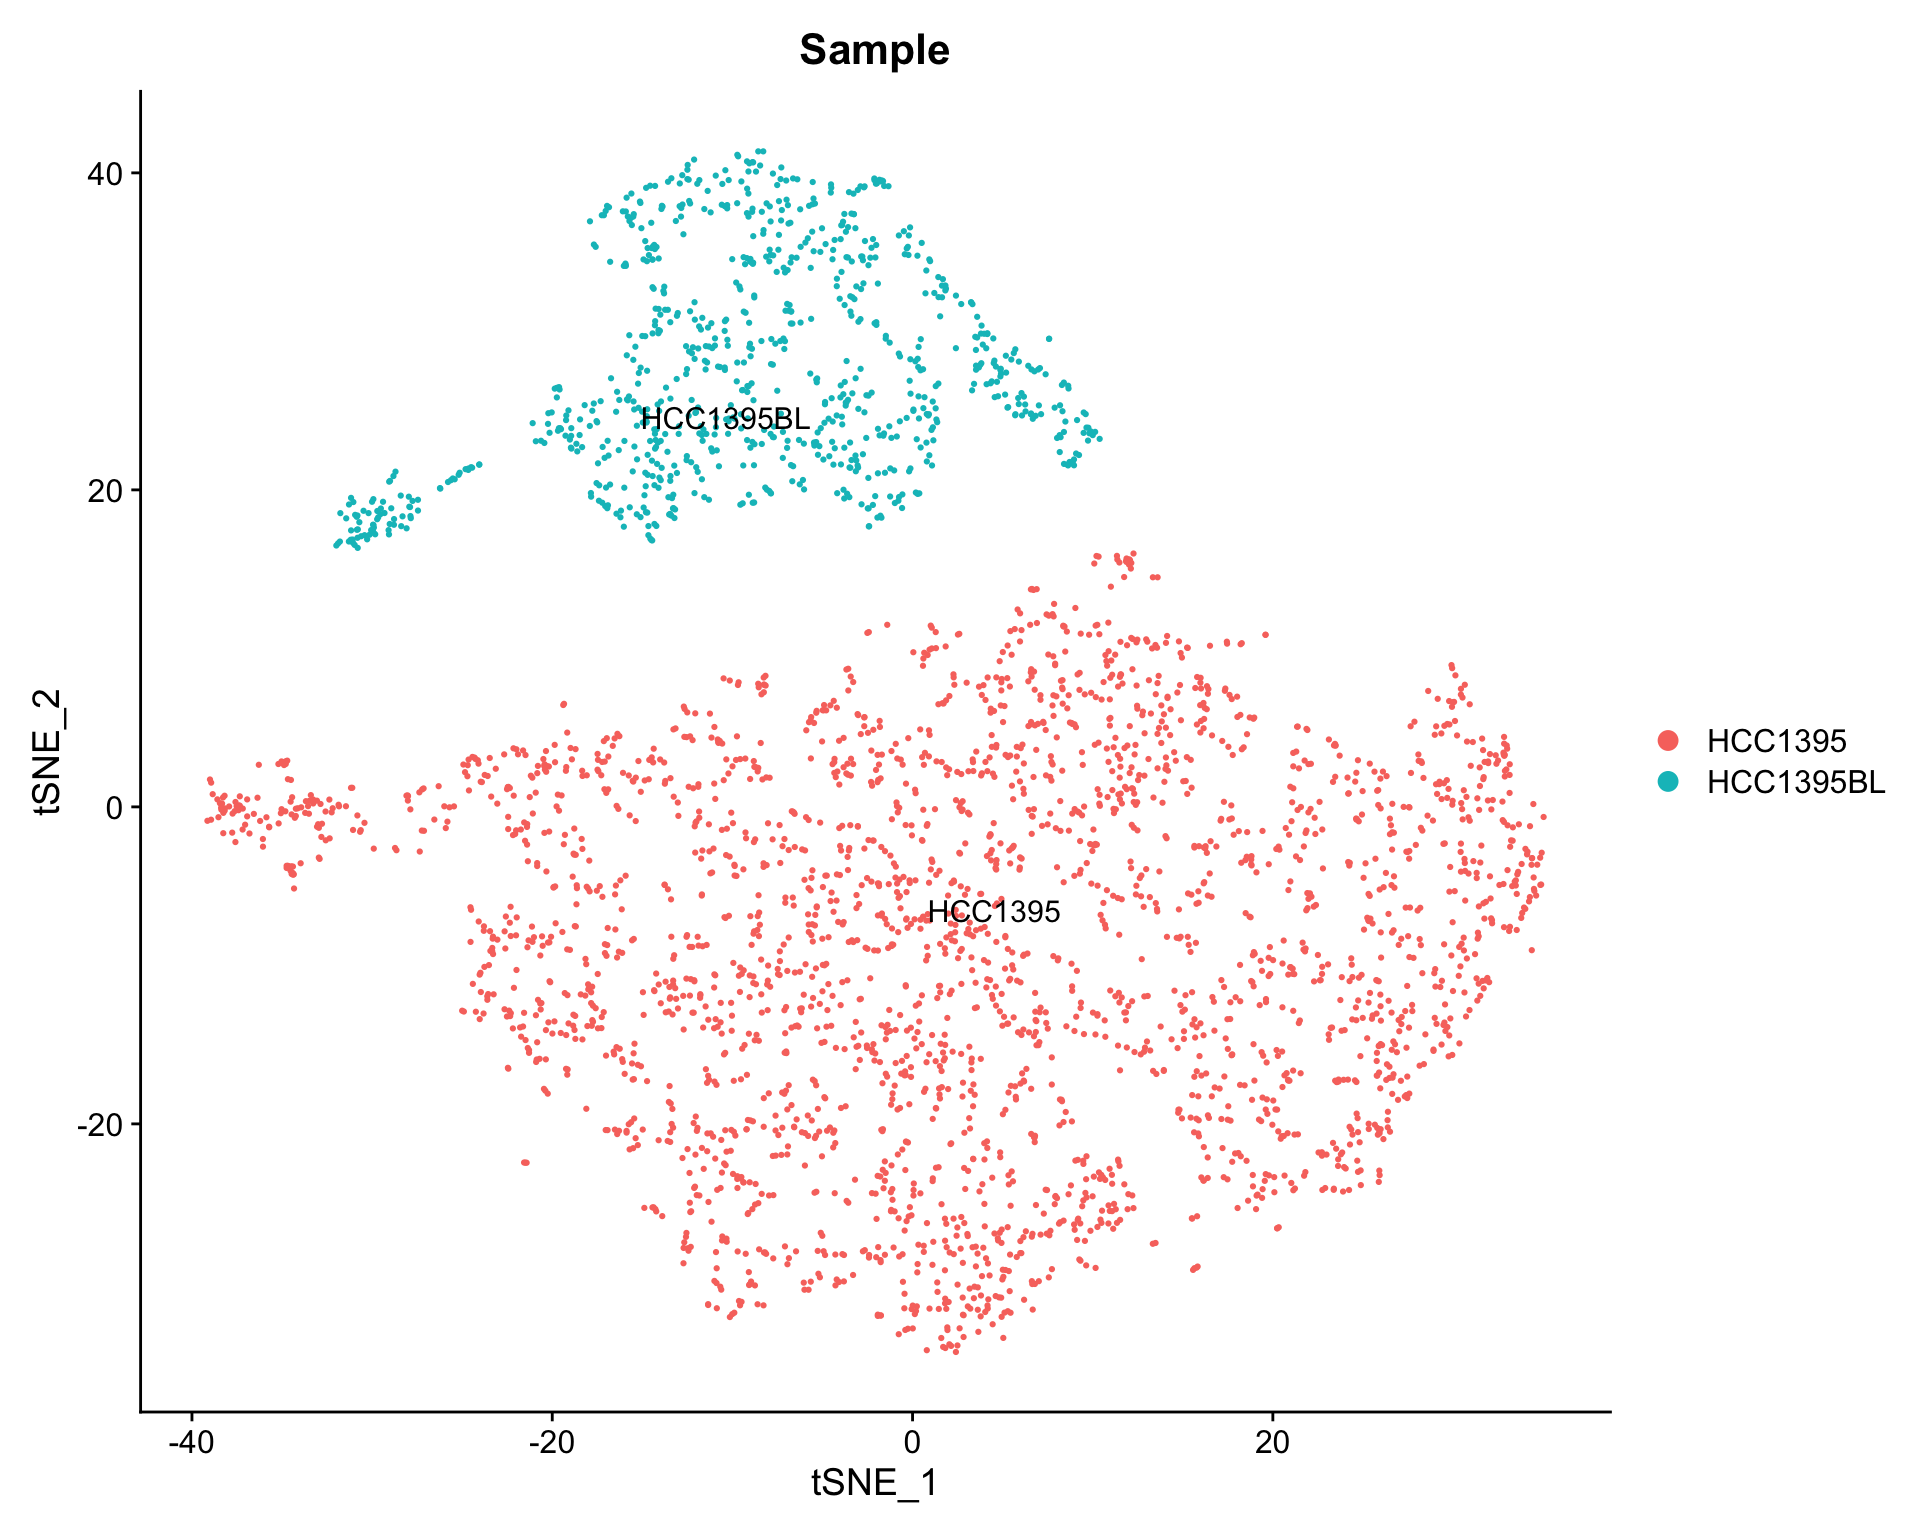
\includegraphics{Bioinfo-figures_files/figure-latex/unnamed-chunk-18-1.pdf}

\clearpage

\hypertarget{umap}{%
\section{uMAP}\label{umap}}

Optionally, we can also perform dimension reductionality reduction using UMAP

\begin{Shaded}
\begin{Highlighting}[]
\FunctionTok{DimPlot}\NormalTok{(}
\NormalTok{  counts\_st,}
  \AttributeTok{reduction =} \StringTok{"umap"}\NormalTok{,}
  \AttributeTok{label =}\NormalTok{ T,}
  \AttributeTok{size =} \FloatTok{0.5}\NormalTok{,}
  \AttributeTok{repel =}\NormalTok{ T,}
  \AttributeTok{cols =} \FunctionTok{DiscretePalette}\NormalTok{(}\FunctionTok{length}\NormalTok{(}\FunctionTok{levels}\NormalTok{(}\FunctionTok{Idents}\NormalTok{(}
\NormalTok{    counts\_st}
\NormalTok{  ))))}
\NormalTok{)}
\end{Highlighting}
\end{Shaded}

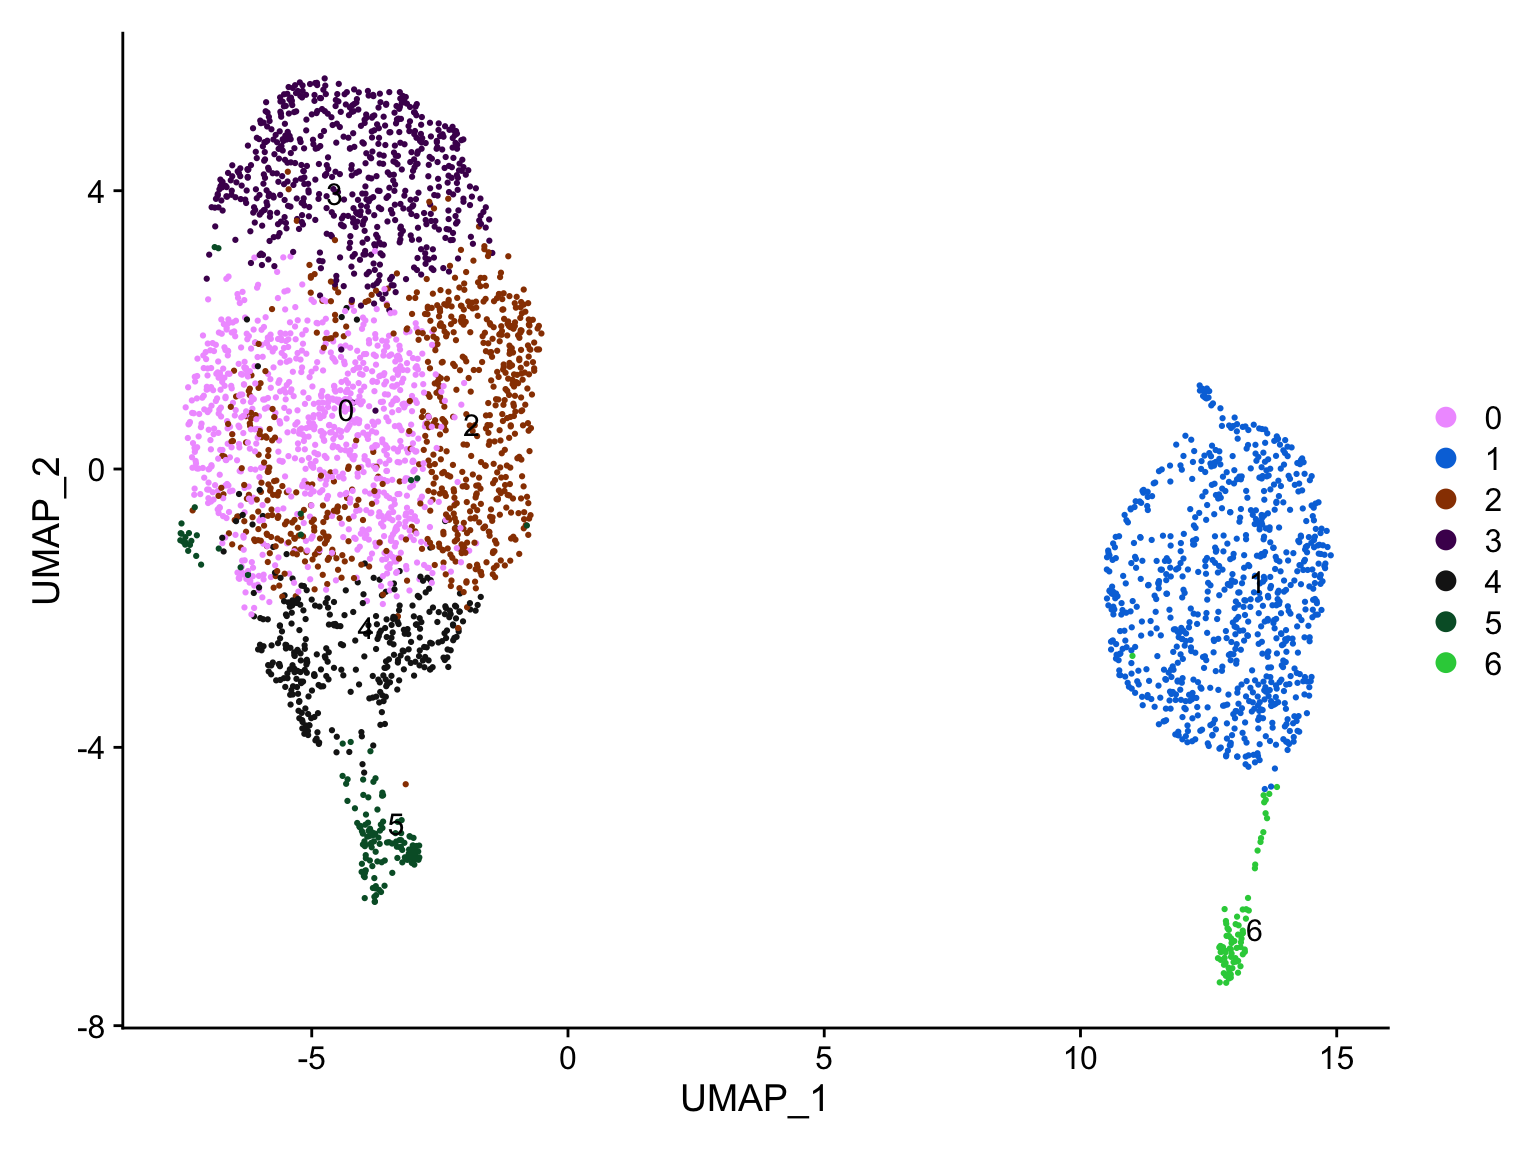
\includegraphics{Bioinfo-figures_files/figure-latex/unnamed-chunk-19-1.pdf}

\begin{Shaded}
\begin{Highlighting}[]
\FunctionTok{DimPlot}\NormalTok{(}
\NormalTok{  counts\_st,}
  \AttributeTok{reduction =} \StringTok{"umap"}\NormalTok{,}
  \AttributeTok{label =}\NormalTok{ T,}
  \AttributeTok{group.by =} \StringTok{"Sample"}\NormalTok{,}
  \AttributeTok{size =} \FloatTok{0.5}\NormalTok{,}
  \AttributeTok{repel =}\NormalTok{ T}
\NormalTok{)}\SpecialCharTok{+}\FunctionTok{ggtitle}\NormalTok{(}\StringTok{""}\NormalTok{)}
\end{Highlighting}
\end{Shaded}

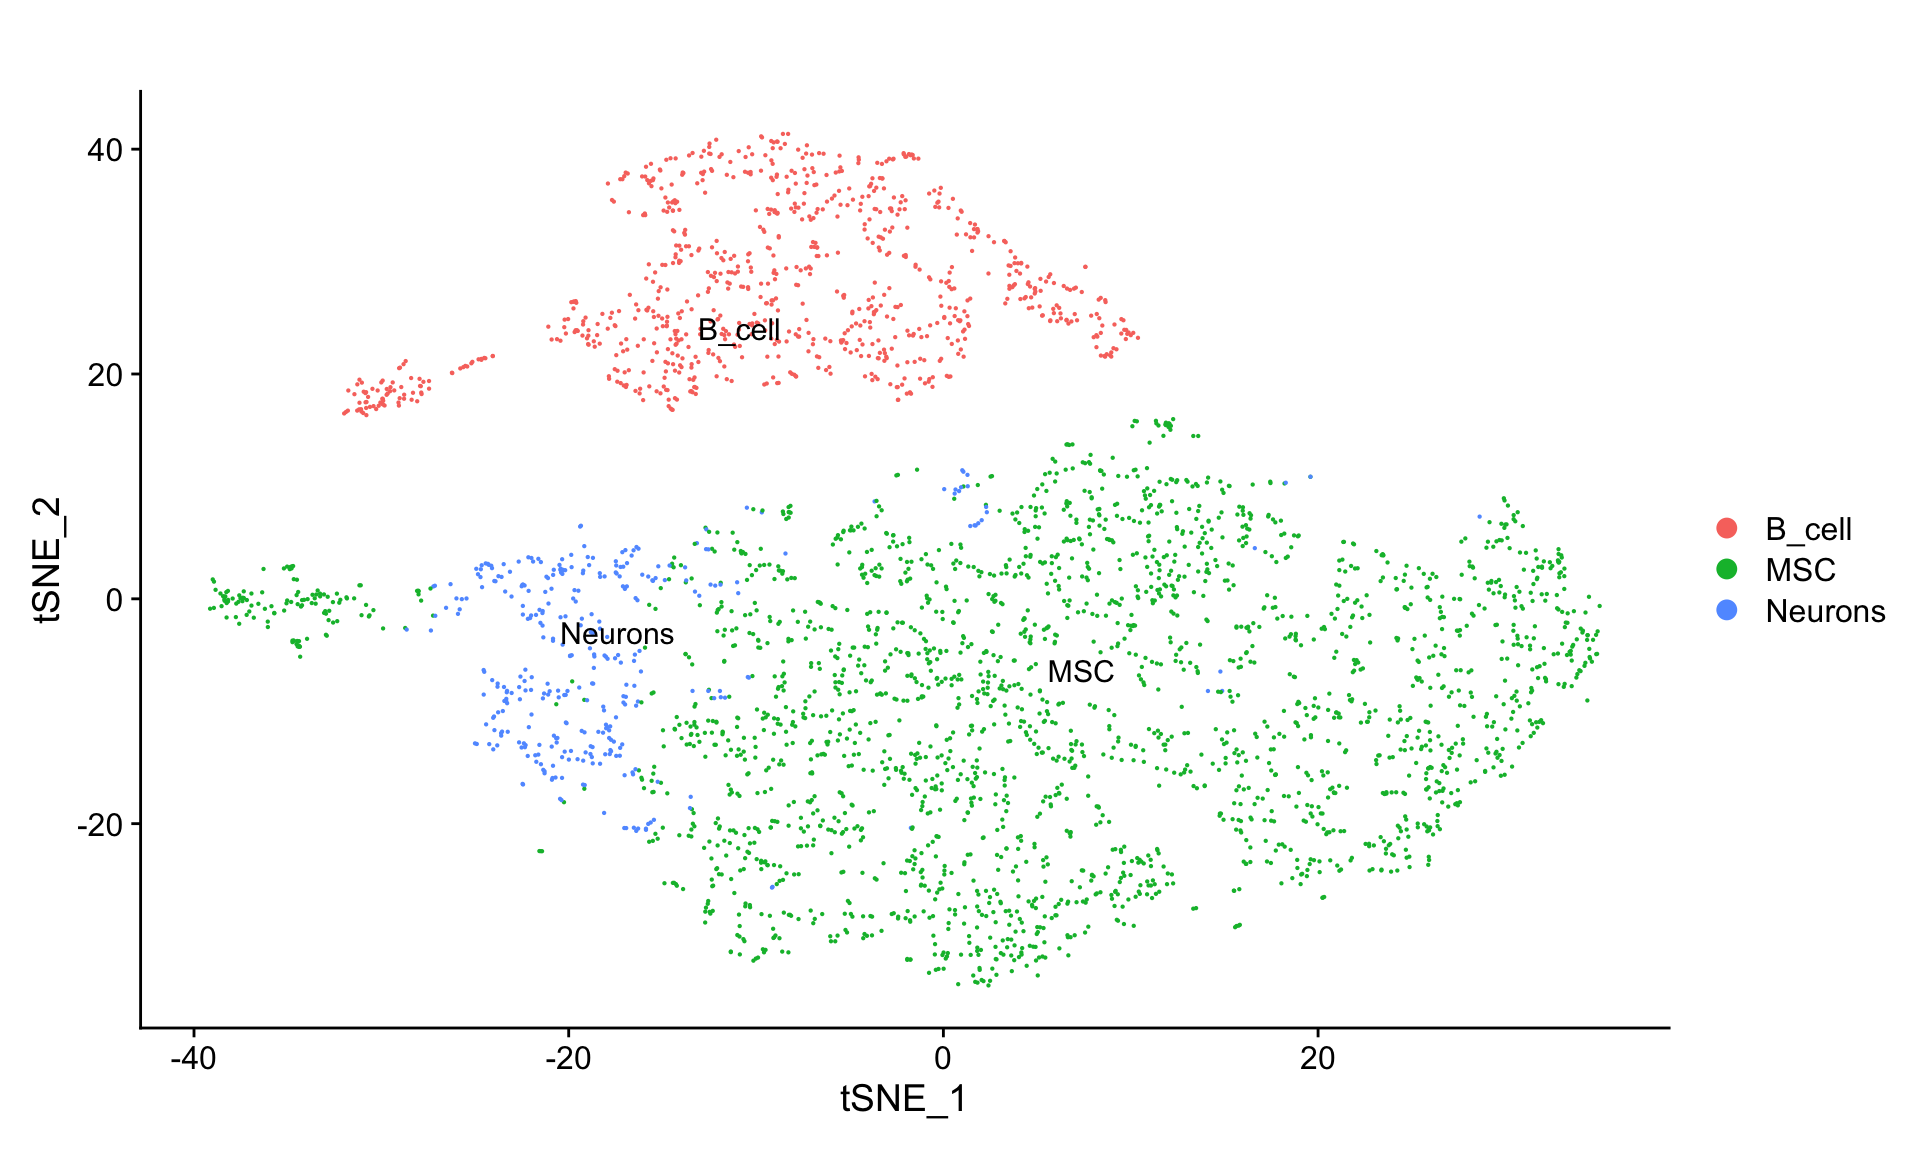
\includegraphics{Bioinfo-figures_files/figure-latex/unnamed-chunk-20-1.pdf}

\clearpage

\hypertarget{differential-expression-analysis-between-clusters}{%
\section{Differential expression analysis between clusters}\label{differential-expression-analysis-between-clusters}}

To identify differentially expressed genes between clusters we can use the \emph{FindMarker} function in Seurat. As an example, DE genes between clusters 0 and 1 are computed below.

\begin{Shaded}
\begin{Highlighting}[]
\NormalTok{DE.cluster0\_1 }\OtherTok{\textless{}{-}} \FunctionTok{FindMarkers}\NormalTok{(}
\NormalTok{  counts\_st,}
 \AttributeTok{ident.1 =} \DecValTok{0}\NormalTok{,}
 \AttributeTok{ident.2 =} \DecValTok{1}\NormalTok{,}
 \AttributeTok{verbose =}\NormalTok{ F)}
\FunctionTok{head}\NormalTok{(DE.cluster0\_1[}\FunctionTok{order}\NormalTok{(}\FunctionTok{abs}\NormalTok{(DE.cluster0\_1}\SpecialCharTok{$}\NormalTok{avg\_log2FC), }
                         \AttributeTok{decreasing =}\NormalTok{ T),])}
\end{Highlighting}
\end{Shaded}

\begin{verbatim}
##                p_val avg_log2FC pct.1 pct.2     p_val_adj
## CD74    0.000000e+00  -5.891577 0.008 1.000  0.000000e+00
## IGHM    0.000000e+00  -5.729445 0.000 0.998  0.000000e+00
## S100A6  0.000000e+00   5.598281 1.000 0.047  0.000000e+00
## TMSB4X 1.657565e-278  -4.911549 0.970 1.000 2.935713e-274
## CCL3   6.580286e-308  -4.861987 0.000 0.945 1.165434e-303
## KRT81  4.273972e-296   4.593045 0.962 0.000 7.569632e-292
\end{verbatim}

\clearpage

\hypertarget{heatmaps-1}{%
\section{Heatmaps}\label{heatmaps-1}}

Marker genes which can be used to uniquely identify each of the clusters are identified using the \emph{FindAllMarkers} function.

\begin{Shaded}
\begin{Highlighting}[]
\FunctionTok{library}\NormalTok{(dplyr)}
\NormalTok{all.markers }\SpecialCharTok{\%\textgreater{}\%}
  \FunctionTok{group\_by}\NormalTok{(cluster) }\SpecialCharTok{\%\textgreater{}\%}
  \FunctionTok{slice\_max}\NormalTok{(}\AttributeTok{n =} \DecValTok{5}\NormalTok{, }\AttributeTok{order\_by =}\NormalTok{ avg\_log2FC)}
\end{Highlighting}
\end{Shaded}

\begin{verbatim}
## # A tibble: 35 x 7
## # Groups:   cluster [7]
##        p_val avg_log2FC pct.1 pct.2 p_val_adj cluster gene   
##        <dbl>      <dbl> <dbl> <dbl>     <dbl> <fct>   <chr>  
##  1 1.61e-155      1.23  0.94  0.525 2.86e-151 0       IGFBP3 
##  2 4.07e- 65      1.17  0.417 0.149 7.21e- 61 0       IGFBP5 
##  3 2.12e-147      1.06  0.998 0.714 3.75e-143 0       TPM1   
##  4 2.31e-202      0.938 0.994 0.869 4.09e-198 0       CSNK2B 
##  5 1.78e-131      0.901 0.998 0.665 3.15e-127 0       TPM2   
##  6 0              4.79  0.998 0.021 0         1       IGHM   
##  7 0              4.63  1     0.037 0         1       CD74   
##  8 0              4.22  0.945 0.015 0         1       CCL3   
##  9 0              4.08  1     0.959 0         1       TMSB4X 
## 10 0              3.48  0.999 0.033 0         1       HLA-DRA
## # ... with 25 more rows
## # i Use `print(n = ...)` to see more rows
\end{verbatim}

\begin{Shaded}
\begin{Highlighting}[]
\NormalTok{top10.markers}\OtherTok{\textless{}{-}}\NormalTok{all.markers }\SpecialCharTok{\%\textgreater{}\%}
    \FunctionTok{group\_by}\NormalTok{(cluster) }\SpecialCharTok{\%\textgreater{}\%}
    \FunctionTok{slice\_max}\NormalTok{(}\AttributeTok{n =} \DecValTok{10}\NormalTok{, }\AttributeTok{order\_by =}\NormalTok{ avg\_log2FC)}
\end{Highlighting}
\end{Shaded}

\begin{Shaded}
\begin{Highlighting}[]
\FunctionTok{DoHeatmap}\NormalTok{(counts\_st, }\AttributeTok{features =}\NormalTok{ top10.markers}\SpecialCharTok{$}\NormalTok{gene)}
\end{Highlighting}
\end{Shaded}

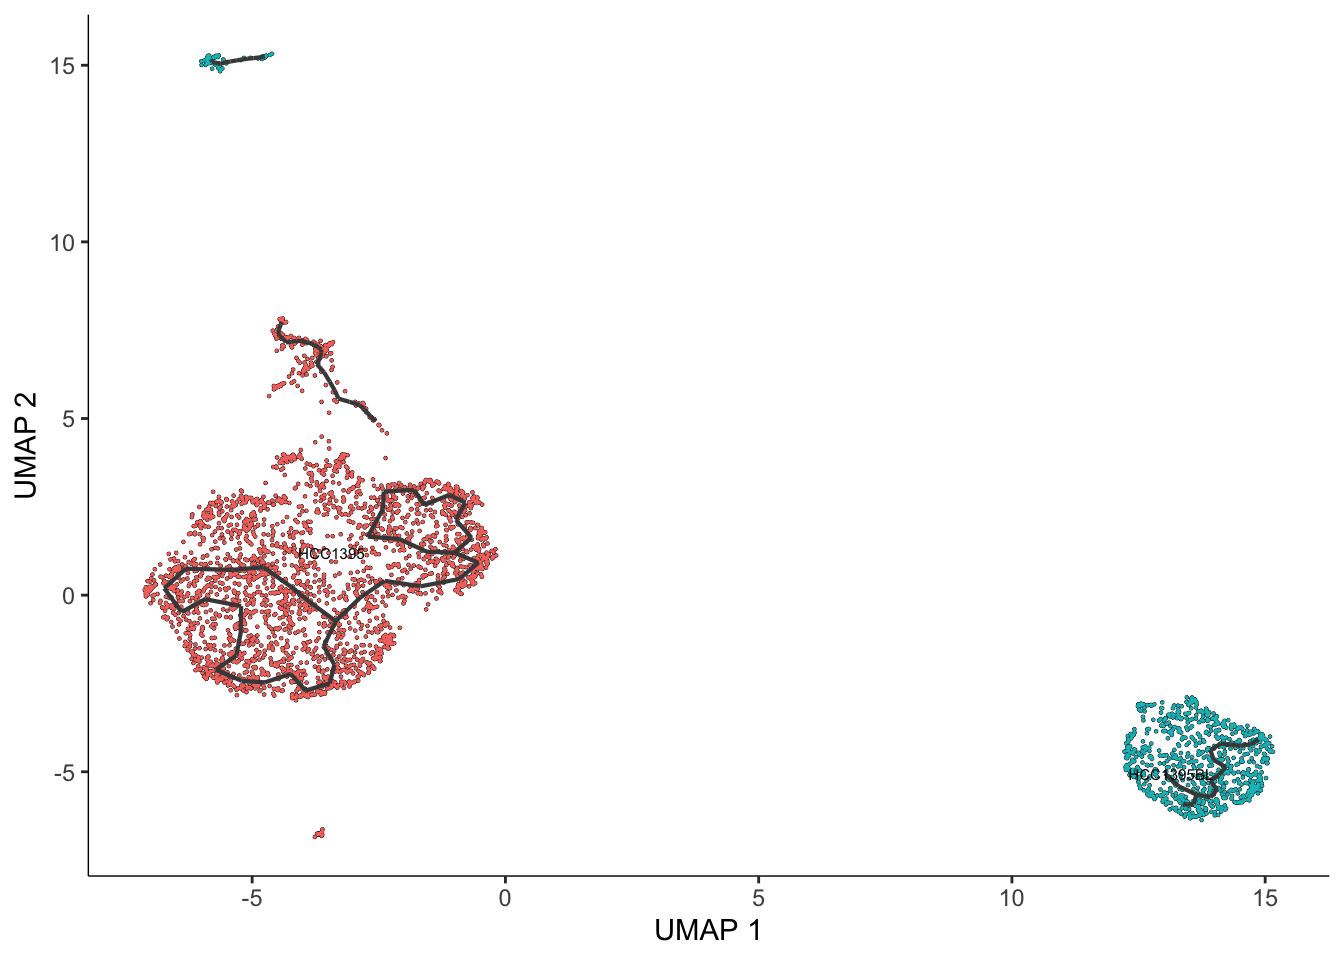
\includegraphics{Bioinfo-figures_files/figure-latex/unnamed-chunk-25-1.pdf}

\clearpage

\hypertarget{feature-plots}{%
\section{Feature plots}\label{feature-plots}}

We can also highlight the expression of genes of interest on the clusters by way of a tSNE plot.

\begin{Shaded}
\begin{Highlighting}[]
\CommentTok{\#Get the top marker gene per cluster}
\NormalTok{top.markers}\OtherTok{\textless{}{-}}\NormalTok{all.markers }\SpecialCharTok{\%\textgreater{}\%}
    \FunctionTok{group\_by}\NormalTok{(cluster) }\SpecialCharTok{\%\textgreater{}\%}
    \FunctionTok{slice\_max}\NormalTok{(}\AttributeTok{n =} \DecValTok{1}\NormalTok{, }\AttributeTok{order\_by =}\NormalTok{ avg\_log2FC)}
\end{Highlighting}
\end{Shaded}

\begin{Shaded}
\begin{Highlighting}[]
\FunctionTok{FeaturePlot}\NormalTok{(}
\NormalTok{  counts\_st,}
  \AttributeTok{features =}\NormalTok{ top.markers}\SpecialCharTok{$}\NormalTok{gene,}
  \AttributeTok{ncol =} \DecValTok{3}\NormalTok{,}
  \AttributeTok{label =}\NormalTok{ T,}
  \AttributeTok{reduction =} \StringTok{"tsne"}
\NormalTok{)}
\end{Highlighting}
\end{Shaded}

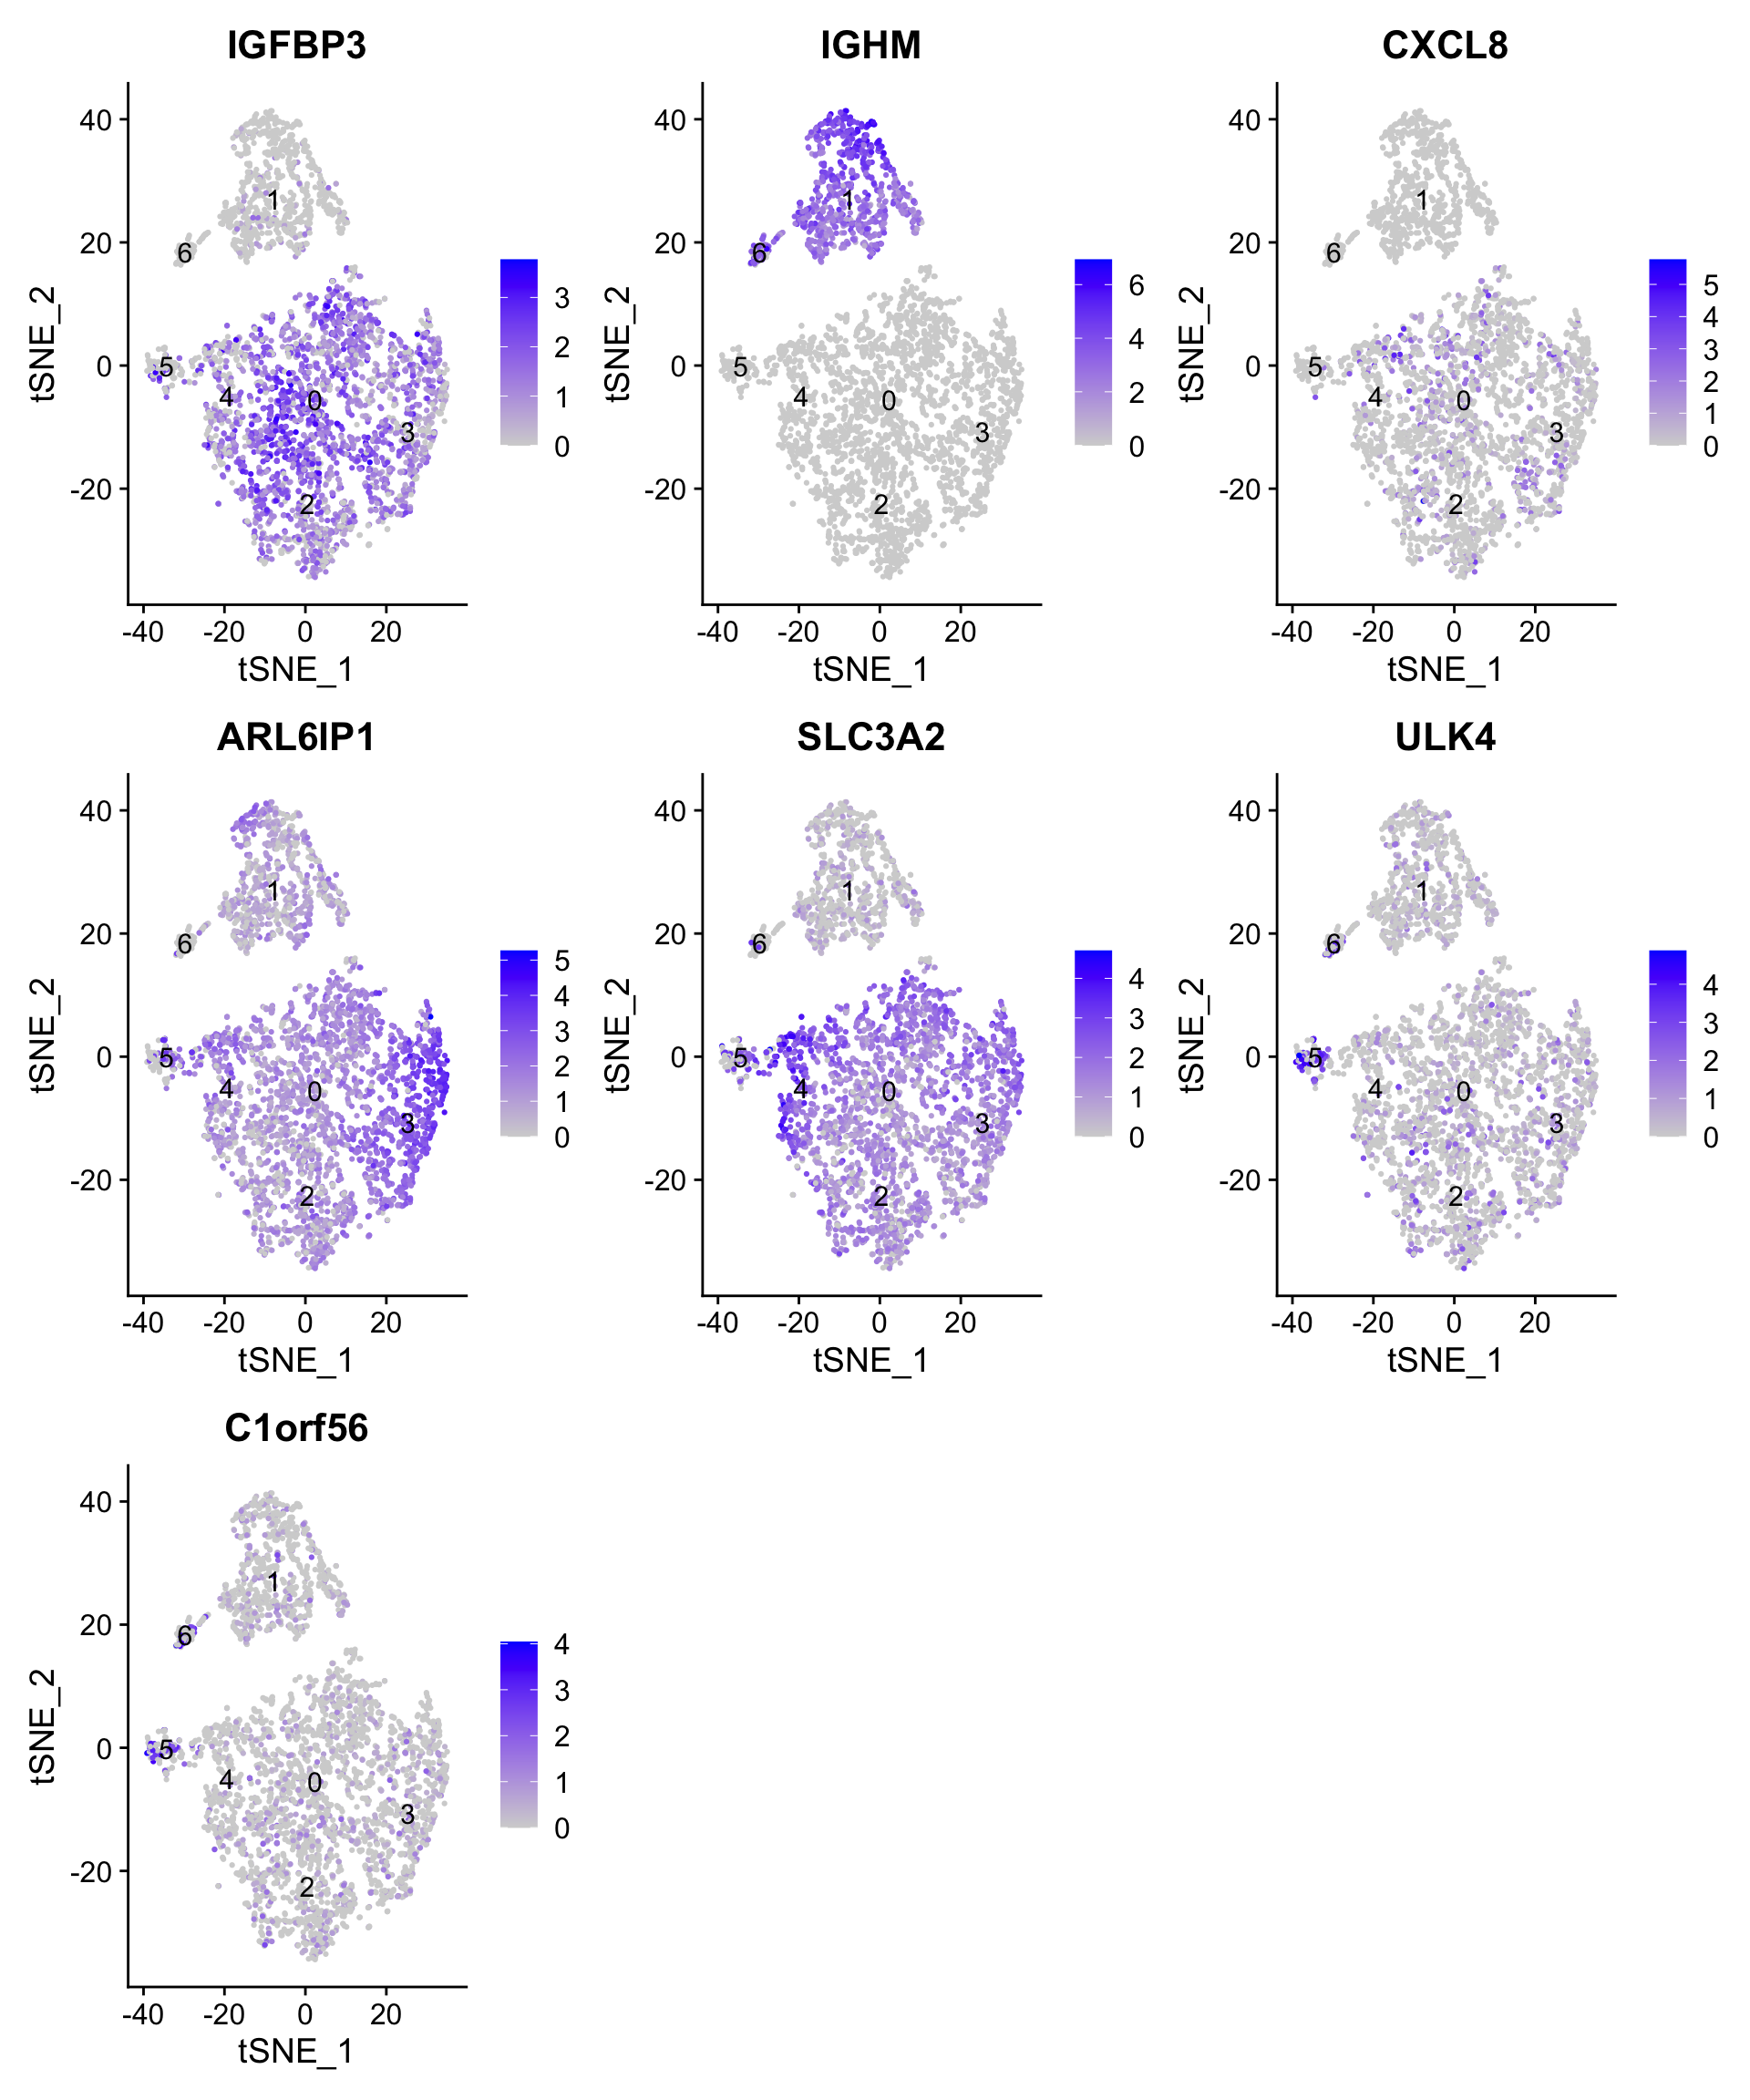
\includegraphics{Bioinfo-figures_files/figure-latex/unnamed-chunk-27-1.pdf}

Alternatively, we can also use violin plots or boxplots to show the expression profile of genes of interest across cells by cluster or any other combination of cells

\begin{Shaded}
\begin{Highlighting}[]
\FunctionTok{VlnPlot}\NormalTok{(counts\_st,}
        \AttributeTok{features =}\NormalTok{ top.markers}\SpecialCharTok{$}\NormalTok{gene,}
        \AttributeTok{cols =} \FunctionTok{DiscretePalette}\NormalTok{(}\FunctionTok{length}\NormalTok{(}\FunctionTok{unique}\NormalTok{(}
\NormalTok{          counts\_st}\SpecialCharTok{$}\NormalTok{seurat\_clusters}
\NormalTok{        ))))}
\end{Highlighting}
\end{Shaded}

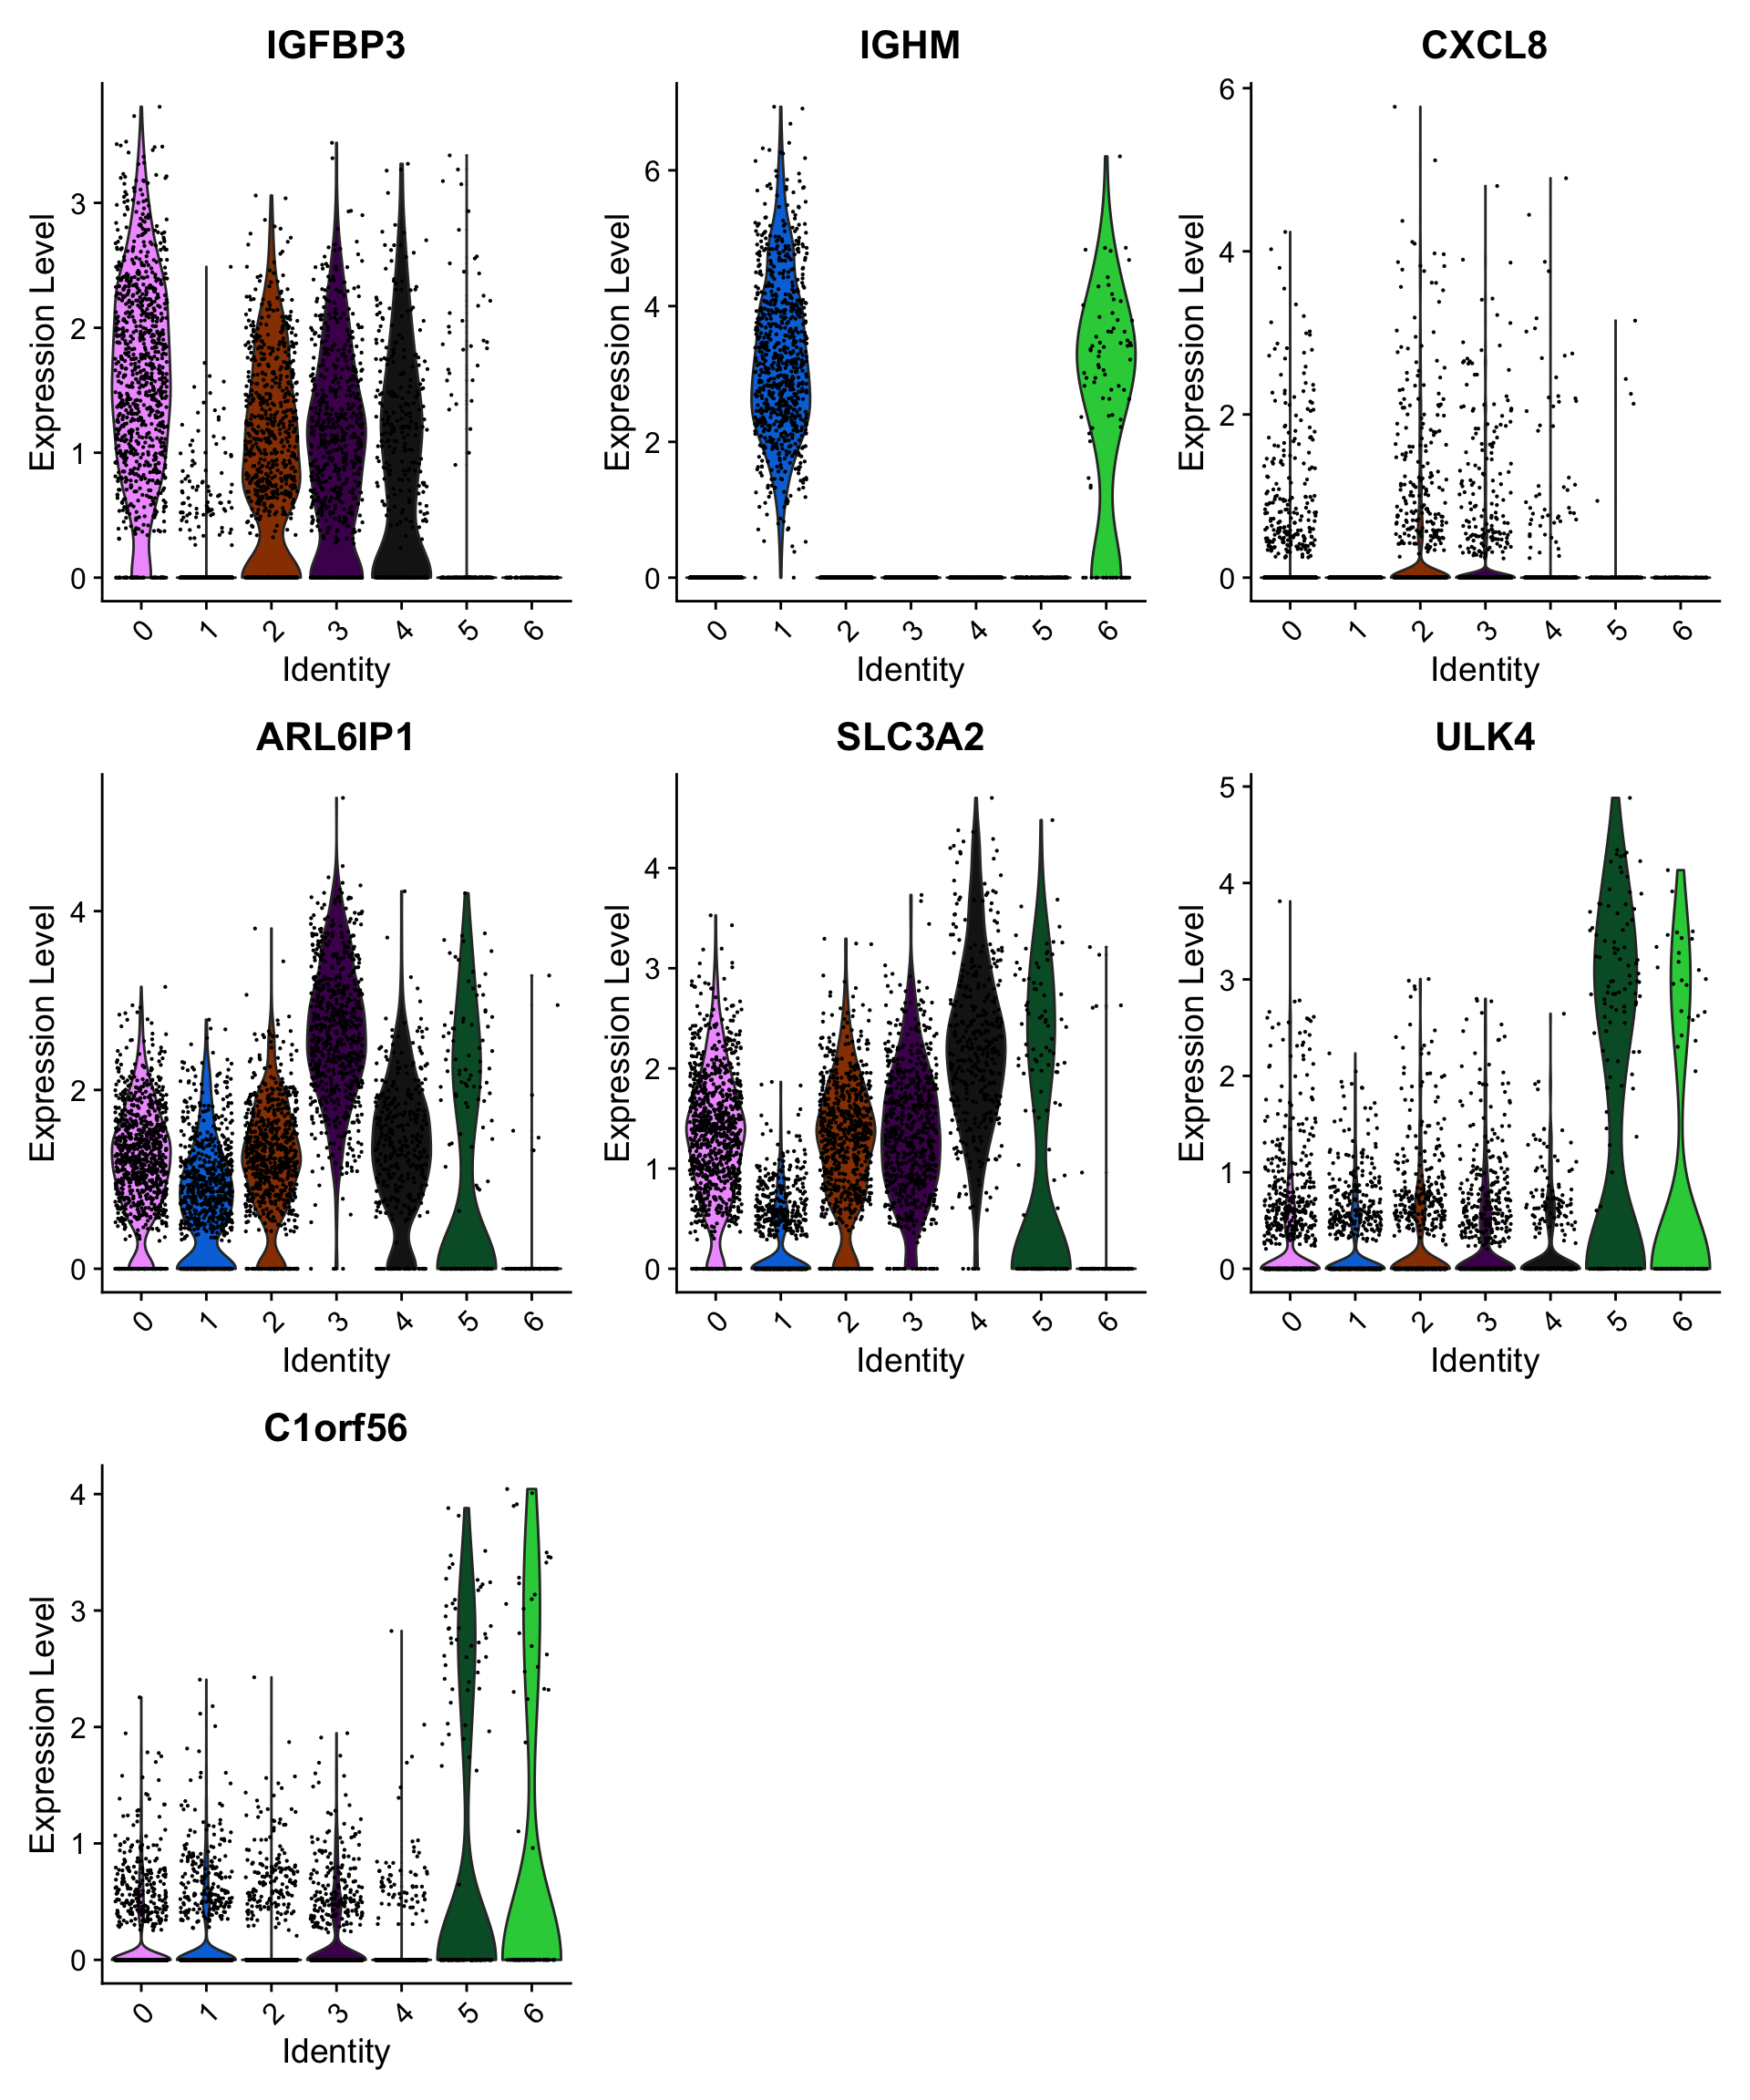
\includegraphics{Bioinfo-figures_files/figure-latex/unnamed-chunk-28-1.pdf}

\begin{Shaded}
\begin{Highlighting}[]
\FunctionTok{par}\NormalTok{(}\AttributeTok{mfrow =} \FunctionTok{c}\NormalTok{(}\DecValTok{3}\NormalTok{, }\DecValTok{3}\NormalTok{))}
\ControlFlowTok{for}\NormalTok{ (n }\ControlFlowTok{in}\NormalTok{ top.markers}\SpecialCharTok{$}\NormalTok{gene)}
\NormalTok{\{}
\NormalTok{  n.data }\OtherTok{\textless{}{-}}\NormalTok{ counts\_st[n, ]}
  \FunctionTok{boxplot}\NormalTok{(}
    \FunctionTok{as.numeric}\NormalTok{(n.data}\SpecialCharTok{@}\NormalTok{assays}\SpecialCharTok{$}\NormalTok{RNA}\SpecialCharTok{@}\NormalTok{data) }\SpecialCharTok{\textasciitilde{}} \FunctionTok{as.character}\NormalTok{(n.data}\SpecialCharTok{$}\NormalTok{seurat\_clusters),}
    \AttributeTok{col =} \FunctionTok{DiscretePalette}\NormalTok{(}\FunctionTok{length}\NormalTok{(}\FunctionTok{unique}\NormalTok{(}
\NormalTok{      counts\_st}\SpecialCharTok{$}\NormalTok{seurat\_clusters}
\NormalTok{    ))),}
    \AttributeTok{xlab =} \StringTok{"Cluster"}\NormalTok{,}
    \AttributeTok{ylab =} \StringTok{"Expression Level"}\NormalTok{,}
    \AttributeTok{main =}\NormalTok{ n}
\NormalTok{  )}
\NormalTok{\}}
\end{Highlighting}
\end{Shaded}

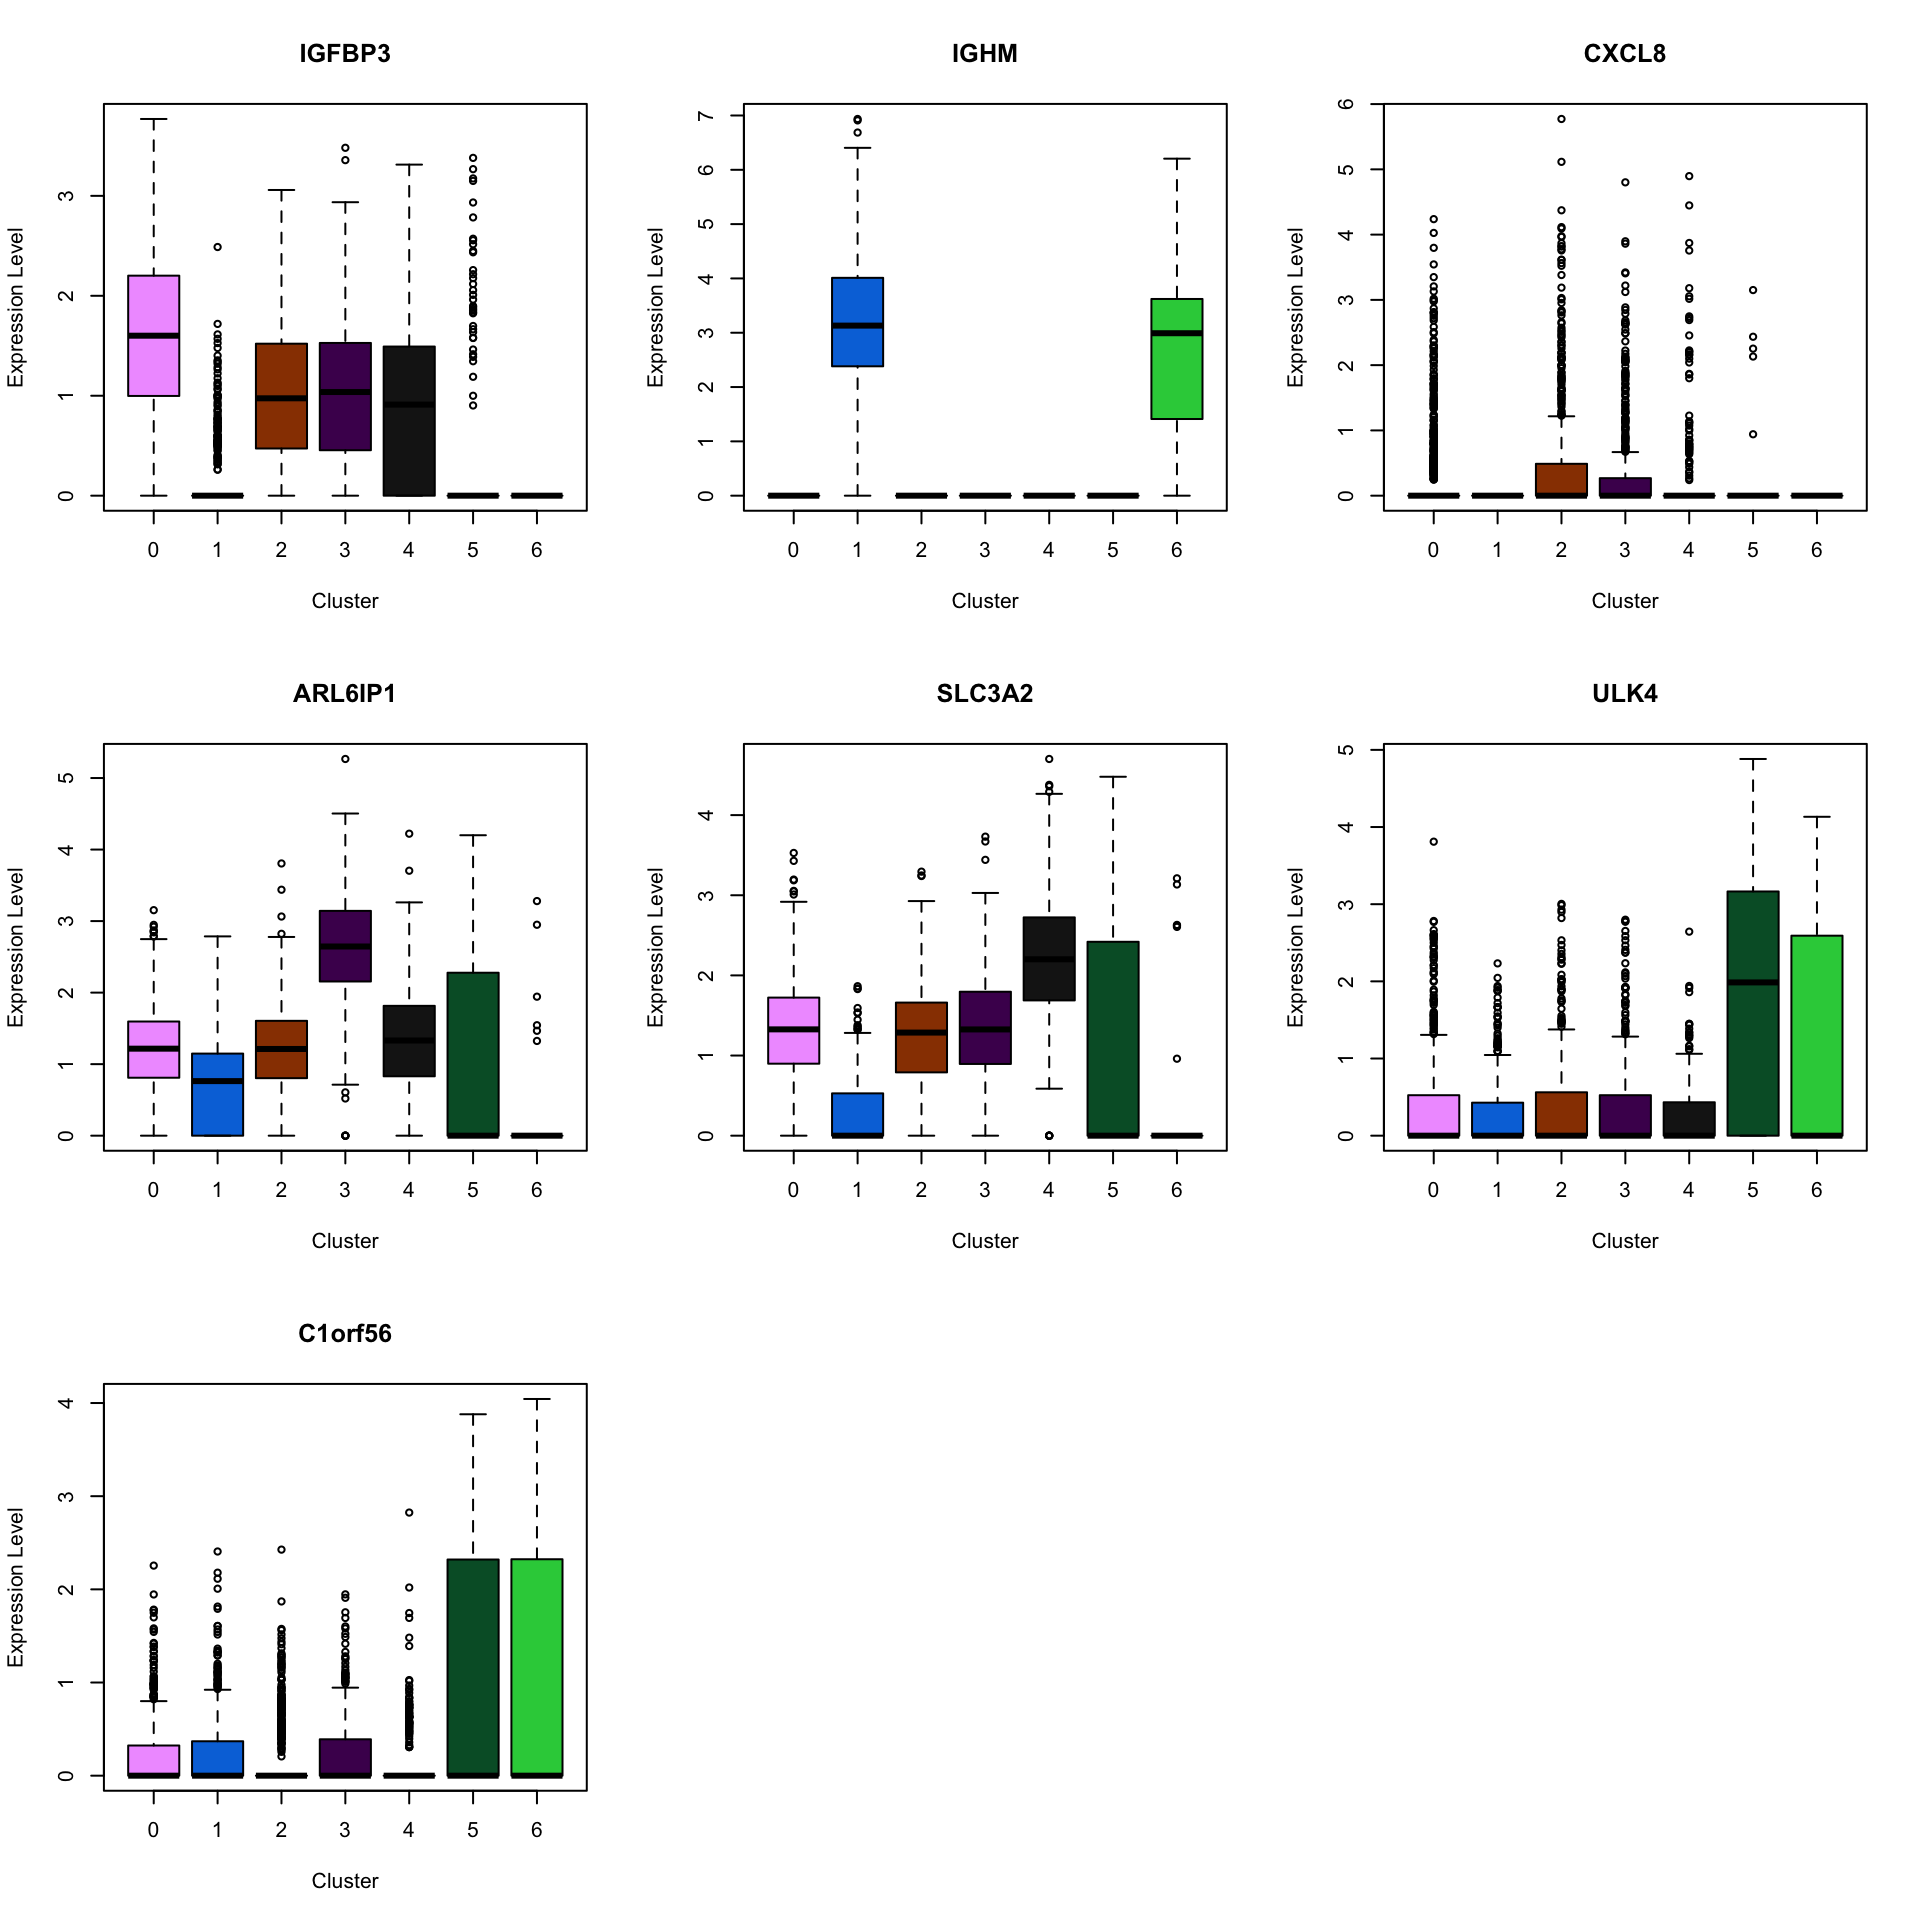
\includegraphics{Bioinfo-figures_files/figure-latex/unnamed-chunk-29-1.pdf}

\clearpage

\hypertarget{cell-annotation}{%
\section{Cell annotation}\label{cell-annotation}}

An unbiased cell type recognition is performed using \textbf{SingleR}. \textbf{celldex} has a range of annotations derived from Bulk RNA-seq data that can be used to annotate the identified clusters above. Here, we use the Human Primary Cell Atlas database as an example.

\begin{Shaded}
\begin{Highlighting}[]
\FunctionTok{library}\NormalTok{(SingleR)}
\FunctionTok{library}\NormalTok{(SingleCellExperiment)}
\end{Highlighting}
\end{Shaded}

\begin{Shaded}
\begin{Highlighting}[]
\NormalTok{cell.sce}\OtherTok{\textless{}{-}} \FunctionTok{as.SingleCellExperiment}\NormalTok{(counts\_st)}
\NormalTok{annot}\OtherTok{\textless{}{-}}\NormalTok{celldex}\SpecialCharTok{::}\FunctionTok{HumanPrimaryCellAtlasData}\NormalTok{()}
\NormalTok{cell.annots }\OtherTok{\textless{}{-}} \FunctionTok{SingleR}\NormalTok{(}
    \AttributeTok{test =}\NormalTok{ cell.sce,}
    \AttributeTok{ref =}\NormalTok{ annot,}
    \AttributeTok{clusters =}\NormalTok{ cell.sce}\SpecialCharTok{$}\NormalTok{seurat\_clusters,}
    \AttributeTok{labels =}\NormalTok{ annot}\SpecialCharTok{$}\NormalTok{label.main)}

\NormalTok{cell.annots.fine}\OtherTok{\textless{}{-}}\FunctionTok{SingleR}\NormalTok{(}
    \AttributeTok{test =}\NormalTok{ cell.sce,}
    \AttributeTok{ref =}\NormalTok{ annot,}
    \AttributeTok{clusters =}\NormalTok{ cell.sce}\SpecialCharTok{$}\NormalTok{seurat\_clusters,}
    \AttributeTok{labels =}\NormalTok{ annot}\SpecialCharTok{$}\NormalTok{label.fine)}

\FunctionTok{save}\NormalTok{(cell.annots,cell.annots.fine,}\AttributeTok{file =} \StringTok{"Annotations.RData"}\NormalTok{)}
\end{Highlighting}
\end{Shaded}

\begin{Shaded}
\begin{Highlighting}[]
\NormalTok{counts\_st }\OtherTok{\textless{}{-}}
  \FunctionTok{AddMetaData}\NormalTok{(counts\_st, cell.annots[}\FunctionTok{match}\NormalTok{(counts\_st}\SpecialCharTok{@}\NormalTok{meta.data}\SpecialCharTok{$}\NormalTok{seurat\_clusters,}\FunctionTok{rownames}\NormalTok{(cell.annots)), }\StringTok{"labels"}\NormalTok{], }\StringTok{"Annot.main"}\NormalTok{)}
\end{Highlighting}
\end{Shaded}

\begin{Shaded}
\begin{Highlighting}[]
\FunctionTok{library}\NormalTok{(ggplot2)}
\end{Highlighting}
\end{Shaded}

\begin{Shaded}
\begin{Highlighting}[]
\FunctionTok{DimPlot}\NormalTok{(}
\NormalTok{    counts\_st,}
    \AttributeTok{reduction =} \StringTok{"tsne"}\NormalTok{,}
    \AttributeTok{group.by =} \StringTok{"Annot.main"}\NormalTok{,}
    \AttributeTok{label =}\NormalTok{ T,}
    \AttributeTok{repel =}\NormalTok{ T,}
    \AttributeTok{pt.size =} \FloatTok{0.1}\NormalTok{,}
\NormalTok{  )}\SpecialCharTok{+}\FunctionTok{ggtitle}\NormalTok{(}\AttributeTok{label =} \StringTok{""}\NormalTok{)}
\end{Highlighting}
\end{Shaded}

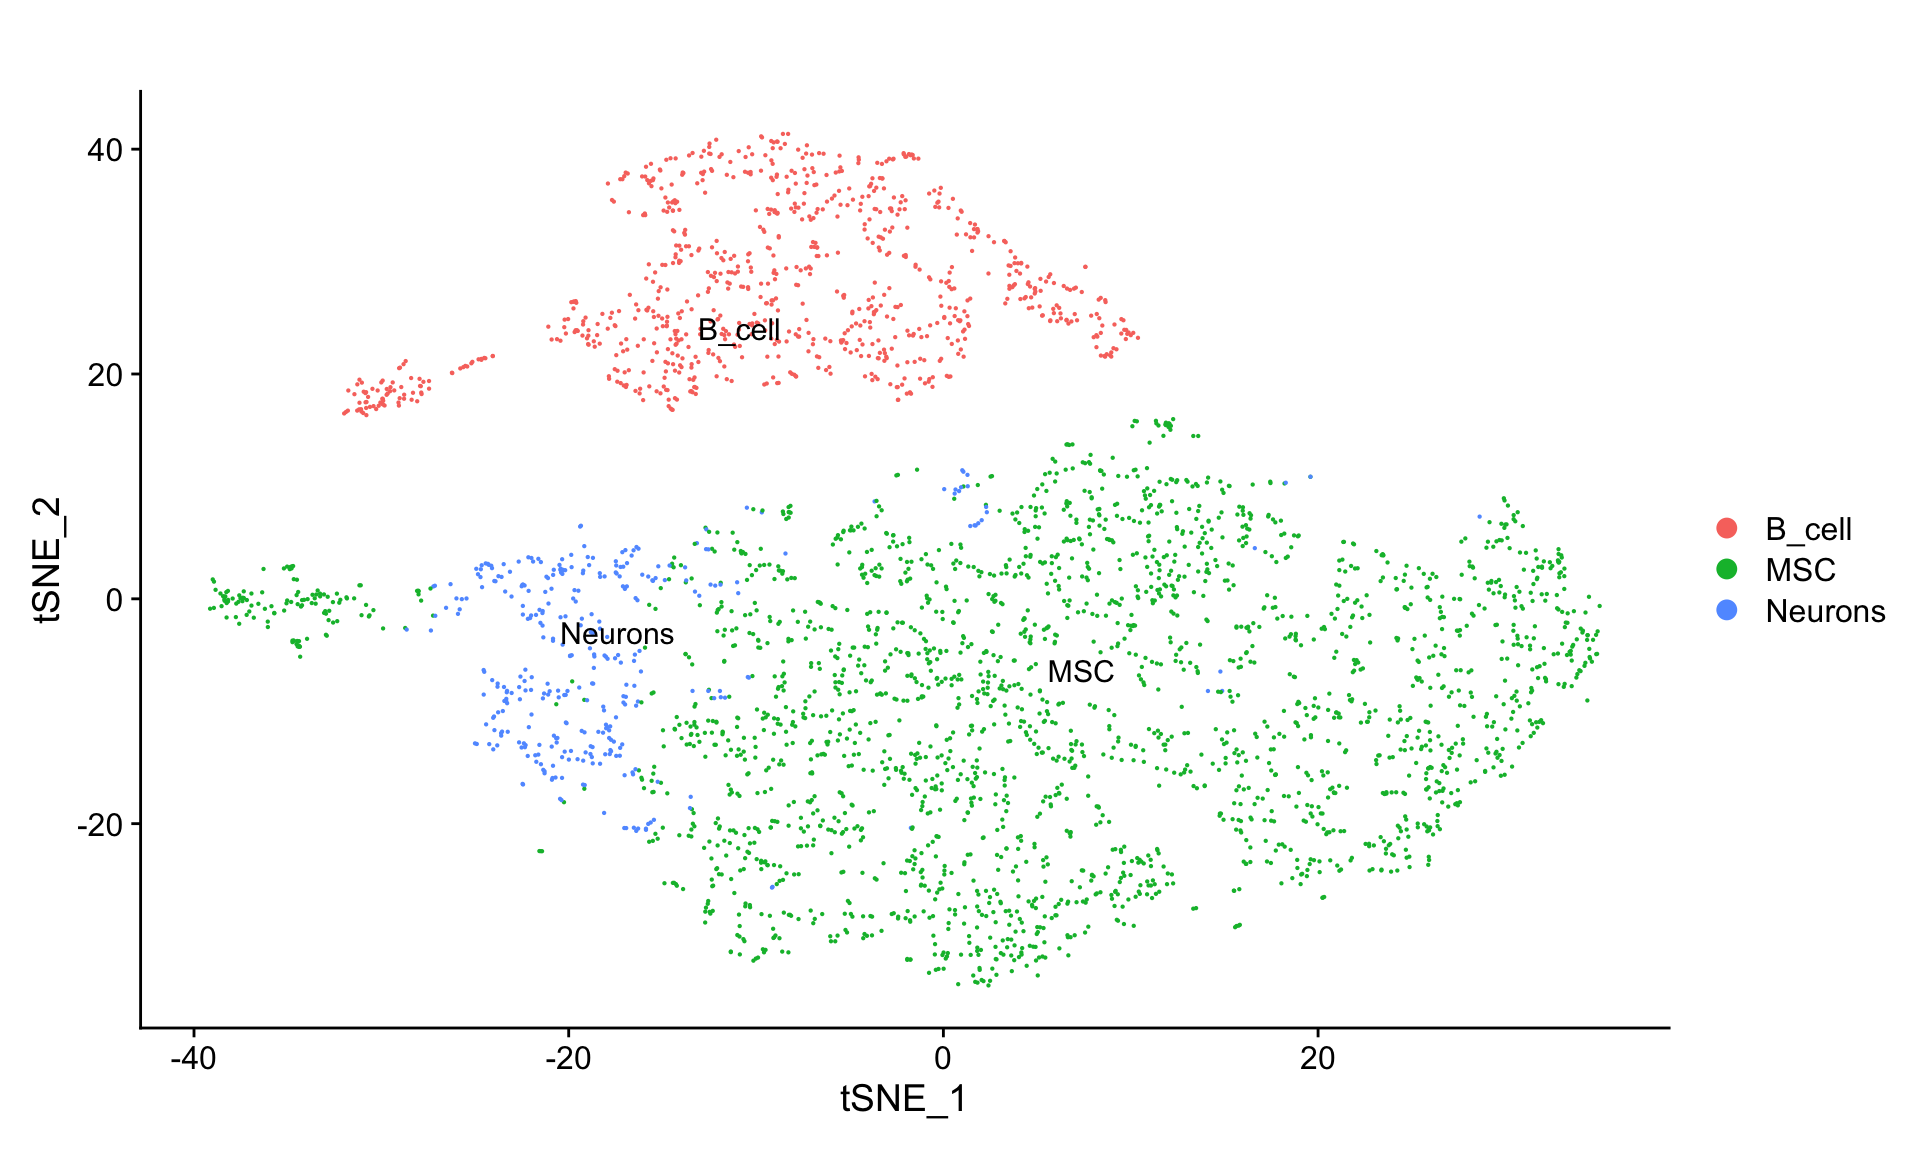
\includegraphics{Bioinfo-figures_files/figure-latex/unnamed-chunk-35-1.pdf}

\begin{Shaded}
\begin{Highlighting}[]
\NormalTok{counts\_st }\OtherTok{\textless{}{-}} \FunctionTok{AddMetaData}\NormalTok{(counts\_st, cell.annots.fine[}\FunctionTok{match}\NormalTok{(counts\_st}\SpecialCharTok{@}\NormalTok{meta.data}\SpecialCharTok{$}\NormalTok{seurat\_clusters, }\FunctionTok{rownames}\NormalTok{(cell.annots.fine)), }\StringTok{"labels"}\NormalTok{], }\StringTok{"Annot.fine"}\NormalTok{)}
\end{Highlighting}
\end{Shaded}

\begin{Shaded}
\begin{Highlighting}[]
\FunctionTok{DimPlot}\NormalTok{(}
\NormalTok{  counts\_st,}
  \AttributeTok{reduction =} \StringTok{"tsne"}\NormalTok{,}
  \AttributeTok{group.by =} \StringTok{"Annot.fine"}\NormalTok{,}
  \AttributeTok{label =}\NormalTok{ T,}
  \AttributeTok{repel =}\NormalTok{ T,}
  \AttributeTok{pt.size =} \FloatTok{0.1}
\NormalTok{) }\SpecialCharTok{+} \FunctionTok{ggtitle}\NormalTok{(}\AttributeTok{label =} \StringTok{""}\NormalTok{)}
\end{Highlighting}
\end{Shaded}

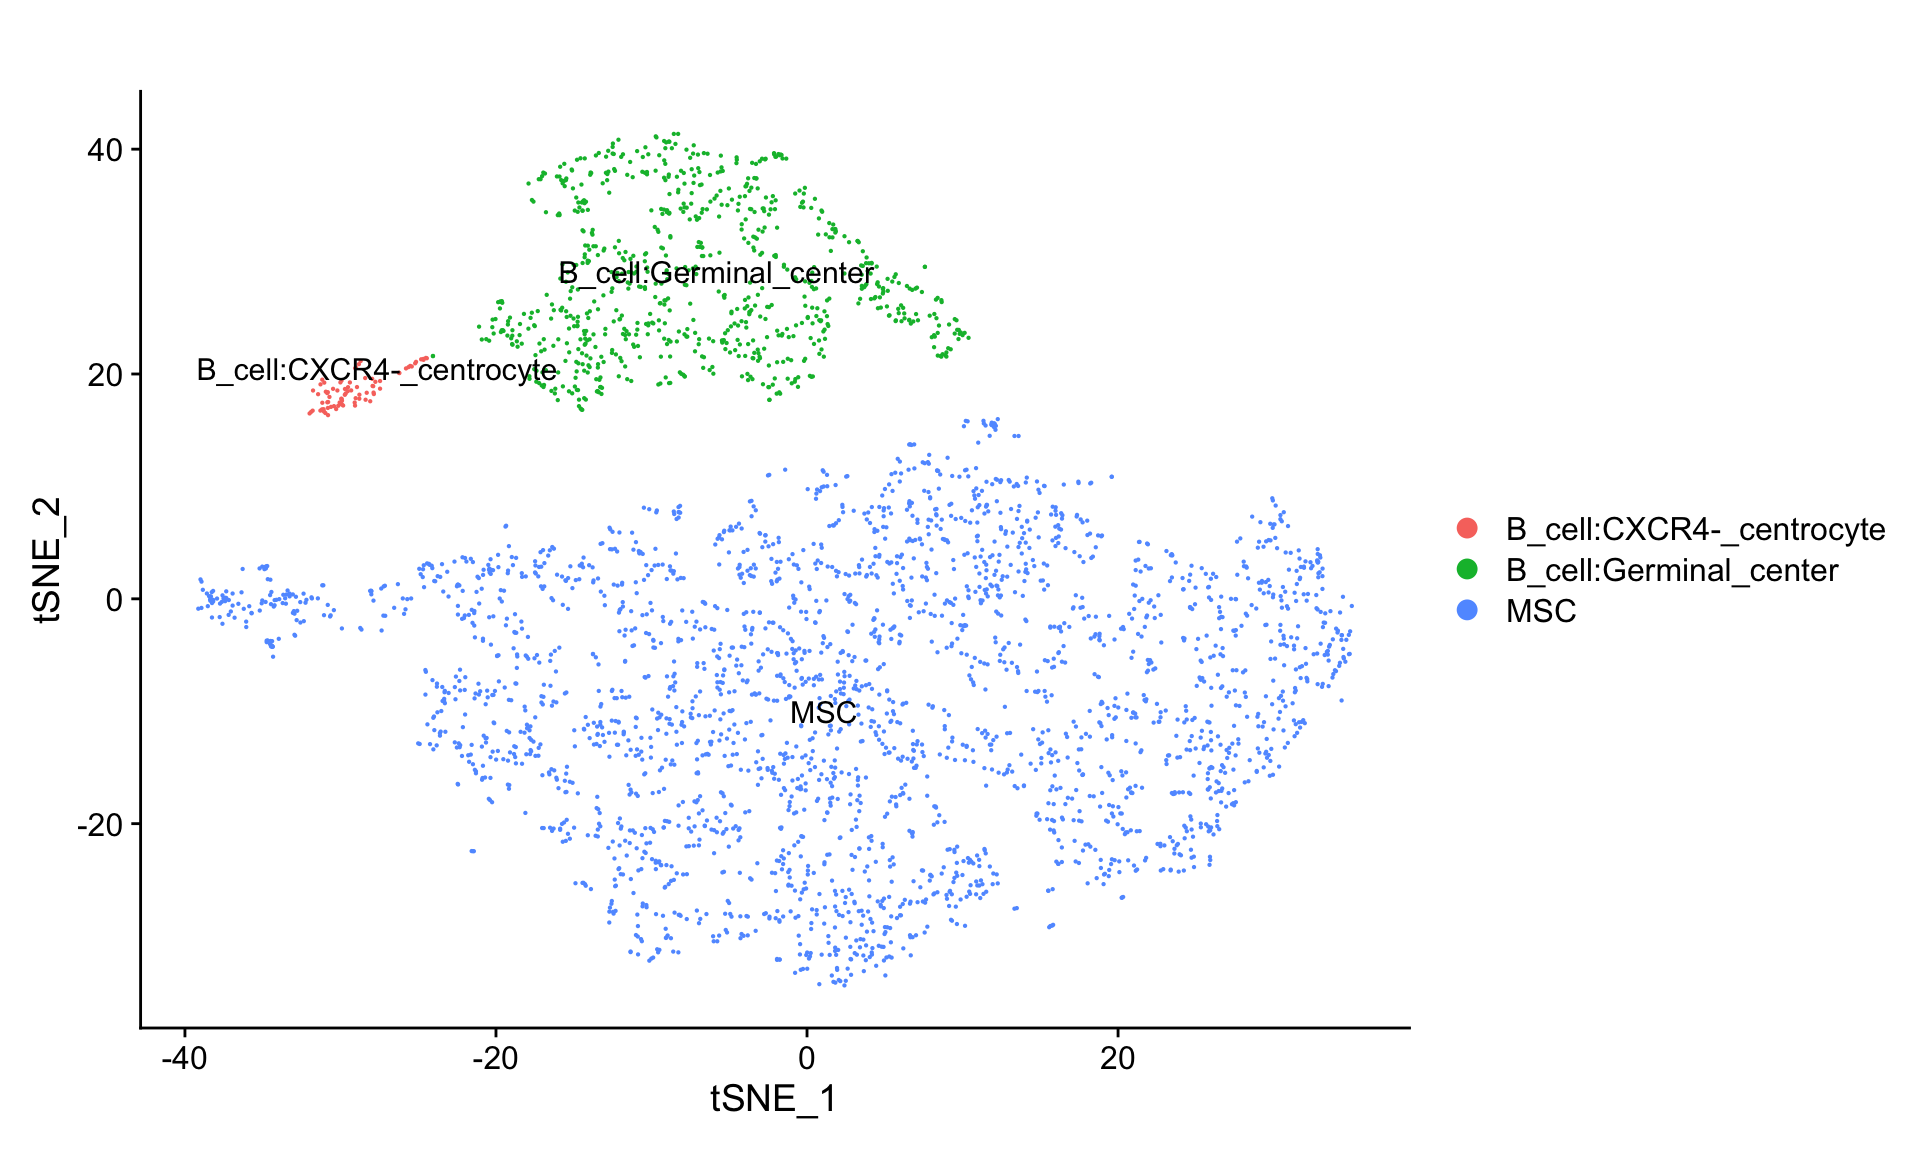
\includegraphics{Bioinfo-figures_files/figure-latex/unnamed-chunk-37-1.pdf}

\clearpage

\hypertarget{trajectory-analysis}{%
\section{Trajectory analysis}\label{trajectory-analysis}}

Pseudotime analysis of the cells identified in the dataset was performed using \textbf{Monocle3}.

\begin{Shaded}
\begin{Highlighting}[]
\NormalTok{mono2.learn.traject }\OtherTok{\textless{}{-}}
  \ControlFlowTok{function}\NormalTok{(X\_counts,}
\NormalTok{           these.cell.types) \{}
    \FunctionTok{library}\NormalTok{(monocle3)}
\NormalTok{    rds.fname }\OtherTok{\textless{}{-}} \StringTok{"Trajectory{-}cds.rds"}
\NormalTok{    gsndf }\OtherTok{\textless{}{-}} \FunctionTok{data.frame}\NormalTok{(}\AttributeTok{gene\_short\_name =} \FunctionTok{rownames}\NormalTok{(X\_counts))}
\NormalTok{    csndf }\OtherTok{\textless{}{-}} \FunctionTok{data.frame}\NormalTok{(}\AttributeTok{cell.type =}\NormalTok{ these.cell.types)}
    \FunctionTok{rownames}\NormalTok{(gsndf) }\OtherTok{\textless{}{-}} \FunctionTok{rownames}\NormalTok{(X\_counts)}
    \FunctionTok{rownames}\NormalTok{(csndf) }\OtherTok{\textless{}{-}} \FunctionTok{colnames}\NormalTok{(X\_counts)}
\NormalTok{    cds }\OtherTok{\textless{}{-}} \FunctionTok{new\_cell\_data\_set}\NormalTok{(}
      \AttributeTok{expression\_data =}\NormalTok{ X\_counts,}
      \AttributeTok{cell\_metadata =}\NormalTok{ csndf,}
      \AttributeTok{gene\_metadata =}\NormalTok{ gsndf}
\NormalTok{    )}
\NormalTok{    cds }\OtherTok{\textless{}{-}} \FunctionTok{preprocess\_cds}\NormalTok{(cds, }\AttributeTok{num\_dim =} \DecValTok{50}\NormalTok{)}
    \CommentTok{\#cds \textless{}{-} align\_cds(cds)}
\NormalTok{    cds }\OtherTok{\textless{}{-}} \FunctionTok{reduce\_dimension}\NormalTok{(cds)}
\NormalTok{    cds }\OtherTok{\textless{}{-}} \FunctionTok{cluster\_cells}\NormalTok{(cds)}
\NormalTok{    cds }\OtherTok{\textless{}{-}} \FunctionTok{learn\_graph}\NormalTok{(cds)}
    \CommentTok{\#cds \textless{}{-} order\_cells(cds)}
    \FunctionTok{saveRDS}\NormalTok{(cds , rds.fname)}
\NormalTok{  \}}
\end{Highlighting}
\end{Shaded}

\begin{Shaded}
\begin{Highlighting}[]
\FunctionTok{mono2.learn.traject}\NormalTok{(}
  \AttributeTok{X\_counts =} \FunctionTok{as.matrix}\NormalTok{(counts\_st}\SpecialCharTok{@}\NormalTok{assays}\SpecialCharTok{$}\NormalTok{RNA}\SpecialCharTok{@}\NormalTok{counts),}
  \AttributeTok{these.cell.types =}\NormalTok{ counts\_st}\SpecialCharTok{$}\NormalTok{Sample}
\NormalTok{)}
\end{Highlighting}
\end{Shaded}

\begin{Shaded}
\begin{Highlighting}[]
\NormalTok{mono.rds }\OtherTok{\textless{}{-}} \FunctionTok{readRDS}\NormalTok{(}\StringTok{"Trajectory{-}cds.rds"}\NormalTok{)}
\NormalTok{monocle3}\SpecialCharTok{::}\FunctionTok{plot\_cells}\NormalTok{(}
\NormalTok{  mono.rds,}
  \AttributeTok{color\_cells\_by =} \StringTok{"cell.type"}\NormalTok{,}
  \AttributeTok{label\_groups\_by\_cluster =} \ConstantTok{FALSE}\NormalTok{,}
  \AttributeTok{label\_leaves =} \ConstantTok{FALSE}\NormalTok{,}
  \AttributeTok{label\_branch\_points =} \ConstantTok{FALSE}
\NormalTok{)}
\end{Highlighting}
\end{Shaded}

\begin{figure}
\centering
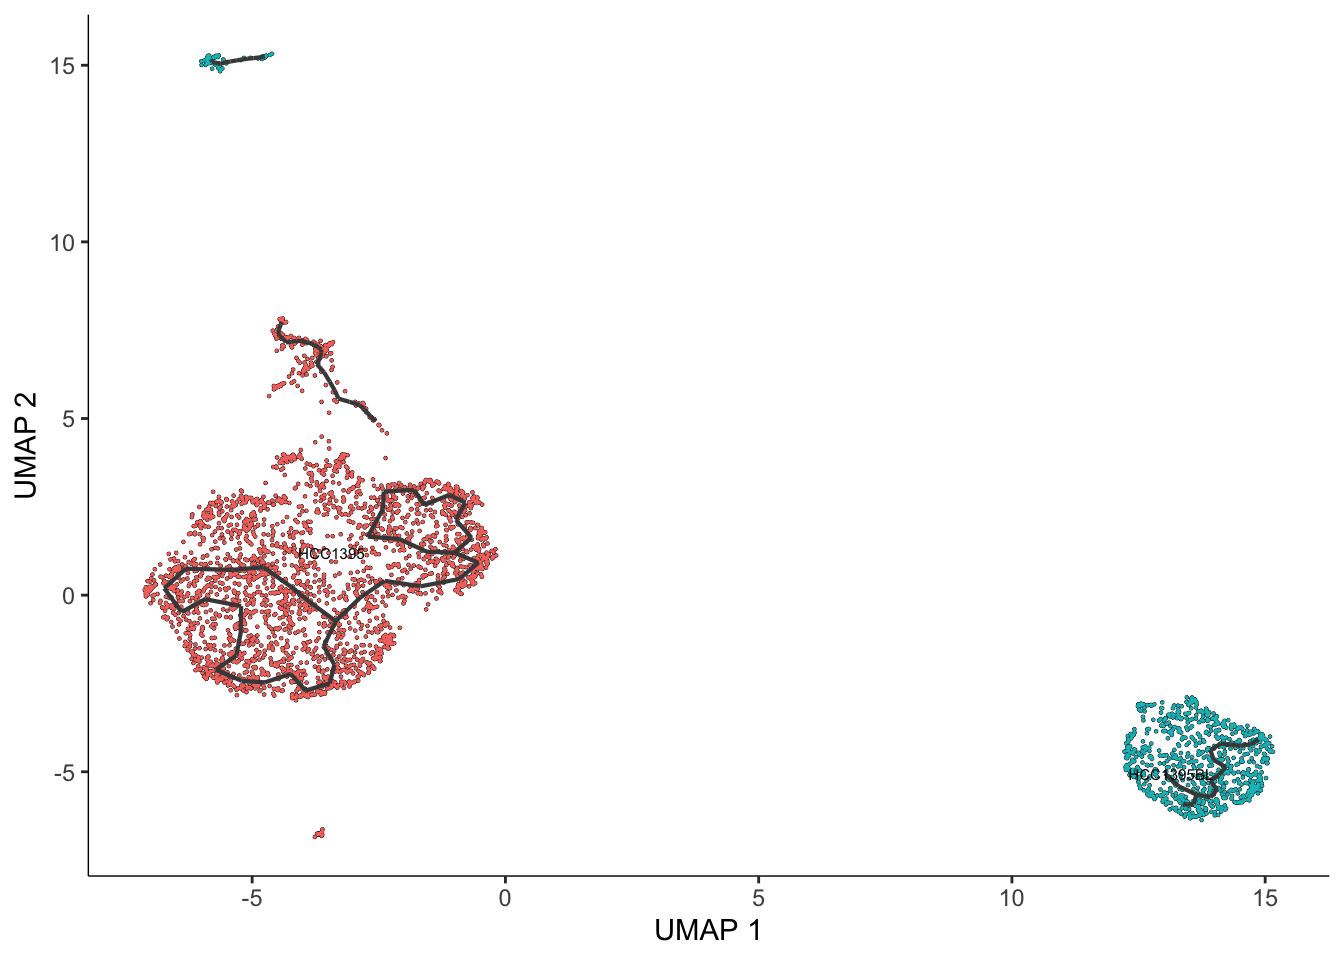
\includegraphics{Bioinfo-figures_files/figure-latex/unnamed-chunk-40-1.pdf}
\caption{\label{fig:unnamed-chunk-40}Pseudo-time plot showing how individual cells progress through the development}
\end{figure}

\clearpage

\textbf{Session info}

\begin{Shaded}
\begin{Highlighting}[]
\FunctionTok{sessionInfo}\NormalTok{()}
\end{Highlighting}
\end{Shaded}

\begin{verbatim}
## R version 4.2.0 (2022-04-22)
## Platform: x86_64-apple-darwin17.0 (64-bit)
## Running under: macOS Big Sur/Monterey 10.16
## 
## Matrix products: default
## BLAS:   /Library/Frameworks/R.framework/Versions/4.2/Resources/lib/libRblas.0.dylib
## LAPACK: /Library/Frameworks/R.framework/Versions/4.2/Resources/lib/libRlapack.dylib
## 
## locale:
## [1] en_AU.UTF-8/en_AU.UTF-8/en_AU.UTF-8/C/en_AU.UTF-8/en_AU.UTF-8
## 
## attached base packages:
## [1] stats4    stats     graphics  grDevices utils     datasets  methods  
## [8] base     
## 
## other attached packages:
##  [1] SingleCellExperiment_1.18.0 SingleR_1.10.0             
##  [3] SummarizedExperiment_1.26.1 GenomicRanges_1.48.0       
##  [5] GenomeInfoDb_1.32.2         MatrixGenerics_1.8.1       
##  [7] matrixStats_0.62.0          dplyr_1.0.9                
##  [9] ggplot2_3.3.6               sp_1.5-0                   
## [11] SeuratObject_4.1.0          Seurat_4.1.1               
## [13] org.Mm.eg.db_3.15.0         GO.db_3.15.0               
## [15] AnnotationDbi_1.58.0        IRanges_2.30.0             
## [17] S4Vectors_0.34.0            Biobase_2.56.0             
## [19] BiocGenerics_0.42.0         Glimma_2.6.0               
## [21] limma_3.52.2               
## 
## loaded via a namespace (and not attached):
##   [1] utf8_1.2.2                reticulate_1.25          
##   [3] lme4_1.1-30               tidyselect_1.1.2         
##   [5] RSQLite_2.2.15            htmlwidgets_1.5.4        
##   [7] grid_4.2.0                BiocParallel_1.30.3      
##   [9] Rtsne_0.16                munsell_0.5.0            
##  [11] ScaledMatrix_1.4.0        codetools_0.2-18         
##  [13] ica_1.0-3                 future_1.27.0            
##  [15] miniUI_0.1.1.1            withr_2.5.0              
##  [17] spatstat.random_2.2-0     colorspace_2.0-3         
##  [19] progressr_0.10.1          highr_0.9                
##  [21] knitr_1.39                rstudioapi_0.13          
##  [23] ROCR_1.0-11               tensor_1.5               
##  [25] listenv_0.8.0             labeling_0.4.2           
##  [27] GenomeInfoDbData_1.2.8    polyclip_1.10-0          
##  [29] bit64_4.0.5               farver_2.1.1             
##  [31] parallelly_1.32.1         vctrs_0.4.1              
##  [33] generics_0.1.3            xfun_0.31                
##  [35] R6_2.5.1                  ggbeeswarm_0.6.0         
##  [37] rsvd_1.0.5                locfit_1.5-9.6           
##  [39] bitops_1.0-7              spatstat.utils_2.3-1     
##  [41] cachem_1.0.6              DelayedArray_0.22.0      
##  [43] assertthat_0.2.1          promises_1.2.0.1         
##  [45] scales_1.2.0              rgeos_0.5-9              
##  [47] beeswarm_0.4.0            gtable_0.3.0             
##  [49] beachmat_2.12.0           globals_0.15.1           
##  [51] goftest_1.2-3             rlang_1.0.4              
##  [53] genefilter_1.78.0         splines_4.2.0            
##  [55] lazyeval_0.2.2            spatstat.geom_2.4-0      
##  [57] yaml_2.3.5                reshape2_1.4.4           
##  [59] abind_1.4-5               httpuv_1.6.5             
##  [61] tools_4.2.0               bookdown_0.27            
##  [63] ellipsis_0.3.2            gplots_3.1.3             
##  [65] spatstat.core_2.4-4       RColorBrewer_1.1-3       
##  [67] ggridges_0.5.3            Rcpp_1.0.9               
##  [69] plyr_1.8.7                sparseMatrixStats_1.8.0  
##  [71] zlibbioc_1.42.0           purrr_0.3.4              
##  [73] RCurl_1.98-1.8            rpart_4.1.16             
##  [75] deldir_1.0-6              pbapply_1.5-0            
##  [77] cowplot_1.1.1             zoo_1.8-10               
##  [79] ggrepel_0.9.1             cluster_2.1.3            
##  [81] magrittr_2.0.3            data.table_1.14.2        
##  [83] scattermore_0.8           lmtest_0.9-40            
##  [85] RANN_2.6.1                fitdistrplus_1.1-8       
##  [87] patchwork_1.1.1           mime_0.12                
##  [89] evaluate_0.15             xtable_1.8-4             
##  [91] XML_3.99-0.10             gridExtra_2.3            
##  [93] compiler_4.2.0            monocle3_1.2.9           
##  [95] tibble_3.1.8              KernSmooth_2.23-20       
##  [97] crayon_1.5.1              minqa_1.2.4              
##  [99] htmltools_0.5.3           mgcv_1.8-40              
## [101] later_1.3.0               tidyr_1.2.0              
## [103] geneplotter_1.74.0        DBI_1.1.3                
## [105] MASS_7.3-58               boot_1.3-28              
## [107] Matrix_1.4-1              cli_3.3.0                
## [109] parallel_4.2.0            igraph_1.3.4             
## [111] pkgconfig_2.0.3           terra_1.5-21             
## [113] plotly_4.10.0             spatstat.sparse_2.1-1    
## [115] annotate_1.74.0           vipor_0.4.5              
## [117] XVector_0.36.0            stringr_1.4.0            
## [119] digest_0.6.29             sctransform_0.3.3        
## [121] RcppAnnoy_0.0.19          spatstat.data_2.2-0      
## [123] Biostrings_2.64.0         rmarkdown_2.14           
## [125] leiden_0.4.2              uwot_0.1.11              
## [127] edgeR_3.38.2              DelayedMatrixStats_1.18.0
## [129] shiny_1.7.2               gtools_3.9.3             
## [131] nloptr_2.0.3              lifecycle_1.0.1          
## [133] nlme_3.1-158              jsonlite_1.8.0           
## [135] BiocNeighbors_1.14.0      viridisLite_0.4.0        
## [137] fansi_1.0.3               pillar_1.8.0             
## [139] lattice_0.20-45           ggrastr_1.0.1            
## [141] KEGGREST_1.36.3           fastmap_1.1.0            
## [143] httr_1.4.3                survival_3.3-1           
## [145] glue_1.6.2                png_0.1-7                
## [147] bit_4.0.4                 stringi_1.7.8            
## [149] blob_1.2.3                DESeq2_1.36.0            
## [151] BiocSingular_1.12.0       caTools_1.18.2           
## [153] memoise_2.0.1             irlba_2.3.5              
## [155] future.apply_1.9.0
\end{verbatim}

\vspace{-100pt}

  \bibliography{Genome.bib,packages.bib}

\end{document}
